\documentclass{sigchi}

% Use this command to override the default ACM copyright statement (e.g. for preprints). 
% Consult the conference website for the camera-ready copyright statement.


%% EXAMPLE BEGIN -- HOW TO OVERRIDE THE DEFAULT COPYRIGHT STRIP -- (July 22, 2013 - Paul Baumann)
\toappear{}
%% EXAMPLE END -- HOW TO OVERRIDE THE DEFAULT COPYRIGHT STRIP -- (July 22, 2013 - Paul Baumann)


% Arabic page numbers for submission. 
% Remove this line to eliminate page numbers for the camera ready copy
% \pagenumbering{arabic}


% Load basic packages
\usepackage{balance}  % to better equalize the last page
\usepackage{graphics} % for EPS, load graphicx instead
\usepackage{times}    % comment if you want LaTeX's default font
\usepackage{url}      % llt: nicely formatted URLs
\usepackage{listings}
\lstset{breaklines}
\usepackage{tabularx}
\usepackage{algpseudocode}
% llt: Define a global style for URLs, rather that the default one
\makeatletter
\def\url@leostyle{%
  \@ifundefined{selectfont}{\def\UrlFont{\sf}}{\def\UrlFont{\small\bf\ttfamily}}}
\makeatother
\urlstyle{leo}


% To make various LaTeX processors do the right thing with page size.
\def\pprw{8.5in}
\def\pprh{11in}
\special{papersize=\pprw,\pprh}
\setlength{\paperwidth}{\pprw}
\setlength{\paperheight}{\pprh}
\setlength{\pdfpagewidth}{\pprw}
\setlength{\pdfpageheight}{\pprh}

% Make sure hyperref comes last of your loaded packages, 
% to give it a fighting chance of not being over-written, 
% since its job is to redefine many LaTeX commands.
\usepackage[pdftex]{hyperref}
\hypersetup{
pdftitle={SIGCHI Conference Proceedings Format},
pdfauthor={LaTeX},
pdfkeywords={SIGCHI, proceedings, archival format},
bookmarksnumbered,
pdfstartview={FitH},
colorlinks,
citecolor=black,
filecolor=black,
linkcolor=black,
urlcolor=black,
breaklinks=true,
}

% create a shortcut to typeset table headings
\newcommand\tabhead[1]{\small\textbf{#1}}


% End of preamble. Here it comes the document.
\begin{document}

\title{Crowdsourcing on In-building Routing System with Personal Preferences across Building Groups}

\numberofauthors{3}
\author{
  \alignauthor Junnan CHEN\\
    \affaddr{Waterloo, Canada}\\
    \email{j486chen@uwaterloo.ca}\\
  \alignauthor Henagzhi ZHANG\\
    \affaddr{Waterloo, Canada}\\
    \email{h246zhang@uwaterloo.ca}\\
}

\maketitle

\begin{abstract}
People travel inside building groups from a room in building A to another in building B frequently. Traditional routing systems usually provide the shortest routes between two coordinates consist of longitudes and latitudes, but do not have knowledge about building structures and detailed floor maps. These systems do not take users' personal preferences into account when suggesting routes as well. Such routes cannot meet people’s demand. In this paper, we introduce a new system, which provides in-building routes based on personal preferences across building groups.
\end{abstract}

\keywords{
	Crowdsourcing; In-building Routing; Personal Preferences; Mobile Interfaces; Concept of Association; Decision Tree.
}

\section{INTRODUCTION}

introduction
In our world, most people are living, working or studying in a group of buildings which could be company buildings, neighborhoods or campus buildings. People go from one location inside the building-group to another every hour every day. Traditional route planning system provides routes between two coordinates consist of longitudes and latitudes, focusing on finding the shortest route, but does not have knowledge about the inside structures of buildings and floor-detailed environments, and does not take users' personal preferences into account when suggesting the routes. Those routes cannot provide enough details and personal options demanded by people.
For example, an employee may need to go to the coffee shop on the first floor of building B from his office on the third floor of building A several times a day. His route choices would be based on the weather condition and his physical condition. He would choose to go through the hallway between the two buildings if it rained or take the elevator if he feels tired. Traditional route planning system would only provide the shortest route from the exit of building B to the entrance of building A regardless of the building structures or floor environments, which cannot meet this employee's actual needs.


Here we want to introduce a new in-building routing system with personal preferences, a system with comprehensive knowledge of building structures, floor-level detailed maps, and relevant environments, which provides room-level detailed routes with personal preferences specified by the user. The focus of this system would be mapping the physical features of routes to human preferences which consist of physical requirement, personal feelings, emotional options and etc. The system shall collect route and preference data from people, and then analyze the relationships between human preferences and physical features.


Our system collects the training data, which are actual routes each has its personal preferences labeled, by crowdsourcing methods. Crowdsourcing has been successfully used in many fields. We provide an application on mobile devices, which encourages people to record their daily routes from one room location to another across building groups. Before they start to record routes, the application will ask the user about their personal feelings today (e.g. Are you hurry now? or Are you feeling tired now?), their special demands for the following route (e.g. Will you pass Tim Hortons on your way? or Do you need to use the bathroom on your way?) as well as some weather conditions (e.g. Is it sunny out side? or Is it snowing now?). Once the users finish the questionaires, they will be presented an interface for them to record their routes. During the recording process, the application collects physical data of the route in the form of points on the floor map inputted by the user. 


Our system will analyze the routes collected and the corresponding physical features of a particular route (e.g. the number of stairs, number of turns) with personal preferences such as physical requirement, personal feelings, and emotional options provided by the user. We will construct our model using the concept of the decision tree. The model is trained by the collected data and will be able to predict the best route given a set of personal preferences.


Our final product aims to generate the proper routes upon request. Using this product, the user could specify two room locations, together with one or more personal preferences. Then, the system will run the model and return the most satisfying route. The system will display the route on the screen for the user. 


In this paper, we describe the design of the crowdsourcing routes collecting method, the feature analyzing method, and route generating system. We test the system with University of Waterloo campus building groups. We provide the test results, the detailed evaluation of our system and the future work.


\section{RELATED WORK}

During the system design process, we reviewed literature related to our ideas. The Kimono ~\cite{huang2005kimono} is a knowledge sharing system, which presents the concept of association. Our in-building routing system uses this idea as well; for example, each route collected in the crowdsourcing stage is associated with a set of personal preferences specified by the user. One of the prior works we reviewed has the similar idea since it ~\cite{heimerl2012communitysourcing} includes a physical kiosk as well. In addition, the physical kiosks ~\cite{heimerl2012communitysourcing} are used for crowdsourcing. Since our system collects in-building routes with personal preferences from our users, crowdsourcing plays a significant role here, and crowdsourcing needs to be studied from the prior work ~\cite{howe2006rise,ipeirotis2014quizz,alt2010location}. Since our system requires users to record routes on the map displayed on the screen and provide inputs through the questionnaire, user interface designs need to be taken into our consideration. Some prior works ~\cite{della2013crowdsourcing,vaataja2011crowdsourced} provide us with very helpful results for our system design. Our results are based on decision trees. In order to have some insights about decision trees, we reviewed and studied related work ~\cite{su2006fast,quinlan1987simplifying}. In this section, we discuss how prior work helps us develop our in-building routing system with personal preferences across building groups. 


\subsection{Concept of Association}

The Kimono paper ~\cite{huang2005kimono} presents a system, which extends the function of an information kiosk. The method they used in order to achieve the extension is to allow interactions between a kiosk and a mobile device, such as a smartphone. We know that a kiosk is usually a physically located machine displaying information. A user could stand in front of a kiosk, and touch the screen to select information of his or her interest. The information from the kiosk is relevant to the particular event at its location. Some disadvantages of a kiosk can be seen. For example, the kiosk lacks mobility, and it’s difficult to add more information to it.


To conquer these inflexibilities, the main idea introduced in the paper ~\cite{huang2005kimono} is to allow interactions between a mobile device (such as a smartphone) and a kiosk. People are familiar with smartphones as they use phones every day. Functionalities of a smartphone include taking pictures, taking notes, recording voices, and so on. Through these various ways, a person can easily create new contents at any time at his or her current location. Then he or she can associate the newly created contents with other selected contents or events presented on the kiosk. By uploading the new contents and its associations, other people can, therefore, have access to them.


The Kimono system ~\cite{huang2005kimono} described in the paper is designed specifically for researchers attending a conference. A number of kiosks are placed in the lobby of the conference. They all display the same information relevant to the event, such as conference locations, routes to the airport, hotels, etc. Changes of talk schedules and meal plans are posted on the kiosks as well. Participants of the conference use the touch panel display of a kiosk to select information interested in. Then the information selected is transferred to his or her smartphone. On the smartphone, the program will alert the user about the next event and other relevant details such as starting/ending time, room location, routes to the destination, etc.


While attending a lecture at the conference, one can use their smartphones to record notes in the form of text, image, video, or audio. Then they associate newly created notes with selected event or items such as papers or posters presented at the conference. People can also exchange notes with each other directly between two mobile devices, or post the notes they took on the kiosk. For those users who previously downloaded information from the kiosk to their smartphones, if the information downloaded has changed, the updates will be copied to the mobile devices through the system when the next synchronization occurs. 


The main insight we learned from the Kimono ~\cite{huang2005kimono} is the concept of associations, which makes the organization of data and synchronization much more simple. Users can get information of his or her interest displayed on the screen and associated information on the smartphone. New information can be created by the user, associated with other relevant information, and made available to others.


For our in-building routing system with personal preferences across building groups, the concept of association is utilized. During the crowdsourcing stage, users record their routes while walking to the destination, and later associate personal preferences or features with the route they just recorded. Personal preferences in our system include physical requirements, personal feelings, emotional options, etc. By associating personal preferences with the routes, the system could provide in-building routes with particular personal preferences specified by a user, and later collect ratings from the user about the routes suggested. 

\subsection{Crowdsourcing}

We can see that a lot of researches and experiments are conducted in prior works ~\cite{heimerl2012communitysourcing,alt2010location} in the area of crowdsourcing. Here we discuss the paper ~\cite{heimerl2012communitysourcing}, in which crowdsourcing concepts are presented and extended as communitysourcing. What we know is that crowdsourcing involves division and assignment of tasks to a number of online users. In order to have better quality work, the kiosk is used to attract the right crowds to perform tasks. In this case, the right crowds are required to be knowledgeable enough in the corresponding task domain assigned to them. The result the paper showed is that the crowdsourcing system was able to perform the grading task more accurately than traditional grading.


What we did is to incorporate the idea of crowdsourcing into our system. That is, we let crowds generate routes with personal preferences through our system. As the system provides in-building routes across building groups on campus, the potential crowds we are interested in are students, teachers, and staffs. One reason is that they are familiar with the building structures and floor-detailed environments, and, therefore, the quality of crowdsourced routes is greatly improved. Another reason is that we could obtain enough route data in a relatively short period of time through the crowdsourcing stage. Furthermore, during the crowdsourcing stage, the system could capture a particular set of preferences associated with a route, and later suggest this route upon requests of same or similar preferences in the set.


\subsection{User Interface}

Since we require the routes to be recorded when users walk to their destinations, our system provides an interface on both computers and mobile devices. The user gets access to our system on the screen in the beginning of his or her journey. Partial map centered at his or her current position is displayed. The user periodically marks his or her next new position along the way to the destination, and the map accordingly centers at the newly marked position. A questionnaire is displayed to request his or her personal preferences associated with the recorded route before the user starts recording.


The questions on the questionnaire are asked before the recording process. The questionnaire of our system helps to collect the personal preference data with the crowdsourced routes of our interest. After thinking of what kinds of questions should be asked, we have the questions such as the weather conditions, the fatigue level, pass coffee shop or not, hurry level, and etc.


When designing such a crowdsourcing interface, we need to think about whether our user interface or task design is effective on both computers and mobile devices. We reviewed the prior paper ~\cite{della2013crowdsourcing} to gain better understandings and insights about crowdsourcing user interfaces and task designs for mobile users.


The main question in the paper ~\cite{della2013crowdsourcing} the author trying to answer is “Which crowdsourcing platforms and which kinds of tasks are more adequate to mobile devices”. It turns out that some of those inadequacy issues are superficial, and they can be resolved by providing better user interfaces and/or better crowdsourcing task designs. Several typical reasons for such inadequacy issues on mobile phones are found as well, such as redundant task description, unsupported formats of audio, scrolling problem, layout problem in a small display, and so on.  


For our system, we also try to conquer these problems by designing simple tasks, requesting simplified inputs, providing concise interfaces, etc. Our system knows the building structures and all of the floor maps. Users records routes through their mobile devices while walking. Partial map centered at the current position is showed, and the user marks the next point along the journey. Upon request of a route with personal preferences specified by a user, the system provides in-building routes and collects ratings for the suggested route afterward. Several benefits can be seen in our system. For example, instead of keeping track of the entire route walked, the user only needs to mark the next new point by touching the screen every time they move as the partial map will always center at his or her current point. After gathering point information inputted by the user, the system itself can generate the corresponding route. By displaying only the partial map instead of the entire floor map, we successfully resolve the bad layout problem on small portable screens.


\subsection{Decision Tree}

Our results are based on decision trees. As described in the previous section, our system provides users with an interface through which users perform question answering and route recording tasks. The system requires users to answer a questionnaire before they start to record their in-building routes during the crowdsourcing stage. The questionnaire here in the system is used to collect personal preference data associated with the routes recorded. And decision trees are then built accordingly. 


We built several graphs of decision trees. What we did was the review of several prior works ~\cite{su2006fast,quinlan1987simplifying} involving the decision trees. A decision tree provides us with support in decision-making. It is known as a tool, which uses a tree-like graph or model of decisions and their possible consequences. A decision tree is a useful technique, which learns a model from a provided data set inductively. In order to build a decision tree, we need to be clear about the structure of a decision tree. The tree structure consists of internal nodes, branches, and leaf nodes. We describe each of the above in turn. Each of the internal nodes is a test on an attribute from our crowdsourced data. Each of the branches represents the result from an internal node. Lastly, a leaf node can be seen as a class label. Three types of nodes are in a decision tree. They are decision nodes, chance nodes, and end nodes. The algorithm is shown to readers through a decision tree. 


Existing algorithms are introduced in early papers ~\cite{breiman1984classification,quinlan1986induction} to help build decision trees. These algorithms ~\cite{breiman1984classification,quinlan1986induction} build decision trees from the given set of training data. Top-down structures are built, partitioning instances into different classes. The splits of instances are based on different attribute values. The algorithm from early work ~\cite{breiman1984classification} uses Gini index to select the splitting attribute. The Gini impurity measures how often a random element from a data set is incorrectly labeled if it was randomly labeled according to the distribution of labels in the subset. Specifically, the Gini impurity is the summation of fi times (1-fi) where fi is the fraction of elements labeled with i.


Decision trees are traditionally drawn manually. However, they can grow to very large trees, which makes it difficult for a person to draw by hand. Here, we used a specialized package in Python to generate decision tree graphs for us. Our goal is to have a model that learns from the data gathered and later makes predictions on some variable of interest. In the graphs we created, colored nodes according to their classes together with explicit variable names are shown. 


Decision trees are commonly utilized in many analytical procedures. What we learned from prior work are a number of advantages of such a decision support technique as follows. For example, a decision tree is relatively easy to understand and interpret, and it requires little data preparation. Furthermore, it allows adding new cases, and can be combined with other decision support techniques. The cost of prediction on a targeted variable using the tree is logarithmic in the training data size.

\section{SYSTEM DESCRIPTON}

Our system is built with knowledge of building structures and floor-level detailed maps of a building group. The main problems that this system is trying to address are collecting routing data with corresponding personal preferences, constructing the routing model based on the collected data. 


The route suggestion problem can be considered as a classification problem. The input data we get from the users are their current status (e.g. if they are tired) and environment conditions (e.g. is it sunny). Our goal is to generate an most suitable route based on all of these variables. For example, if the users are tired, a route using elevators should be more suitable than one which uses stairs intuitively. Since most of the status and conditions we currently consider, like if the user is tired or if the user needs to use a printer, are discrete variables. Taking this into considerations, we determine that a decision tree should be a good option.


\subsection{Basic workflow}

Our basic workflow of the modeling procedure is shown in Figure~\ref{fig:systemflow}

\begin{figure}[!h]
\centering
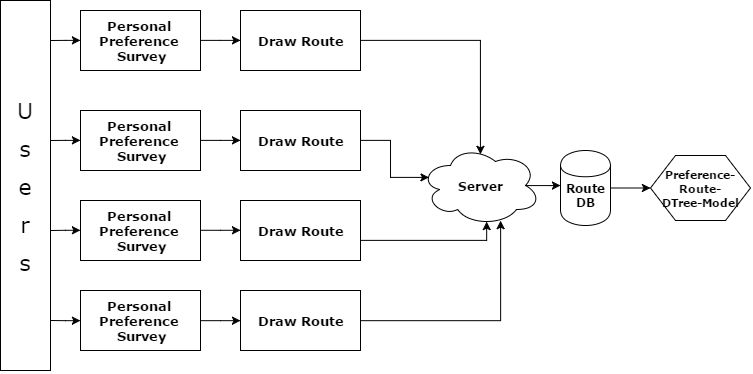
\includegraphics[width=1.0\columnwidth]{pics/work-flow.png}
\caption{System flow chart}
\label{fig:systemflow}
\end{figure}

The modeling procedure mainly consists of two parts:
\begin{itemize}
\item Training data collecting - Crowdsourcing
\item Decision tree constructing
\end{itemize}

\subsection{Training data collecting - Crowdsourcing}

To build a model for the route suggestion problem, we first need to collect data for training decision trees by taking advantage of crowdsourcing.


Crowdsourcing basically has two aspects, to break a large-scaled complex problem into several pieces of sub-problems, and to involve human efforts to solve or help solve the sub-problems which could be time saving because the solving of sub-problems are highly paralleled. Therefore, we found crowdsourcing has the properties which fit the demand of our system perfectly. In the data collection process, we apply crowdsourcing concept by having our participants to record the routes and score the preference options for that route.


The training data collection contains two steps:
\begin{itemize}
\item Survey - Uses are asked to finish a survey about their status and environment conditions.
\item Route drawing - Users are asked to draw a path based their answers to the former survey.
\end{itemize}

\subsubsection{Survey}

The questions and possible answers are in the survey are listed in table~\ref{table:survey_questions}. We convert these answers to a preference vector. From the table, we can see that the values of each element of the vector are discrete. The questions list are far from complete. One potential future work is that we can add more questions based on users’ feedback in crowdsourcing.
\begin{table}
  \centering
  \caption{Survey questions and answers}
  \label{table:survey_questions}
  \begin{tabularx}{0.5\textwidth}{|X|l|}
    \hline \hline
    Questions & Answers \\\hline
    Is it sunny outside? & Yes/NO \\\hline
    Is it cloudy outside? & Yes/NO \\\hline
    Is it rainy/snowy outside? & Yes/NO \\\hline
    Do you feel tired now? & Yes/NO \\\hline
    Do you want to go to Tim Hortons on your way? & Yes/NO \\\hline
    Do you want to go to the bathroom on your way? & Yes/NO \\\hline
    Do you want to avoid crowds at a particular time (e.g. heavy crowds outside MC2065 when class ends, crowds when special events take place, etc.)? & Yes/NO \\\hline
    Are you curious of the floor environment (e.g. first time visit, etc.)? & Yes/NO \\\hline
    Do you need the printer on your way? & Yes/NO \\\hline
    Are you hurry or not through this walk? & Yes/NO \\\hline
    Do you want some fresh air on your way? & Yes/NO \\\hline
    \hline
  \end{tabularx}
\end{table}

\subsubsection{Route drawing}

The users are asked to draw the routes on the maps of each floor. On each map, we marked some special places, like the restrooms, Tim Hortons etc. These marks can help users to plan their route according to their answers (e.g. if they want to grab a cup of coffee). After the users finished their drawing, we will store this route in our server. The route data is in JSON format. One example is:

\begin{verbatim}
"data":{
  "paths":[
    [
      {
        "mapURL":"maps/dc1.png",
        "pointList":[{"x":1,"y":1}]
      },
      {
        "mapURL":"maps/dc2.png",
        "pointList":[{"x":2,"y":2}]
      }
    ]
  ],
  "id":["1449207710639"]
}
\end{verbatim}

After that, we will do analysis on the route data. We analyze each route to derive several physical properties:
\begin{itemize}
\item Number of stairs
\item Times of using elevators
\item Times of exiting buildings
\item If going near Tim Hortons
\item If going near a printer
\item If going a restroom
\item The distance
\item If the route never goes outside
\end{itemize}

A vector of the eight properties is called a physical property vector. A physical property vector should be related to the preference vector.


In summary, for each user, the data we collect is illustrated in Figure~\ref{fig:element-detail}.

\begin{figure}[!h]
\centering
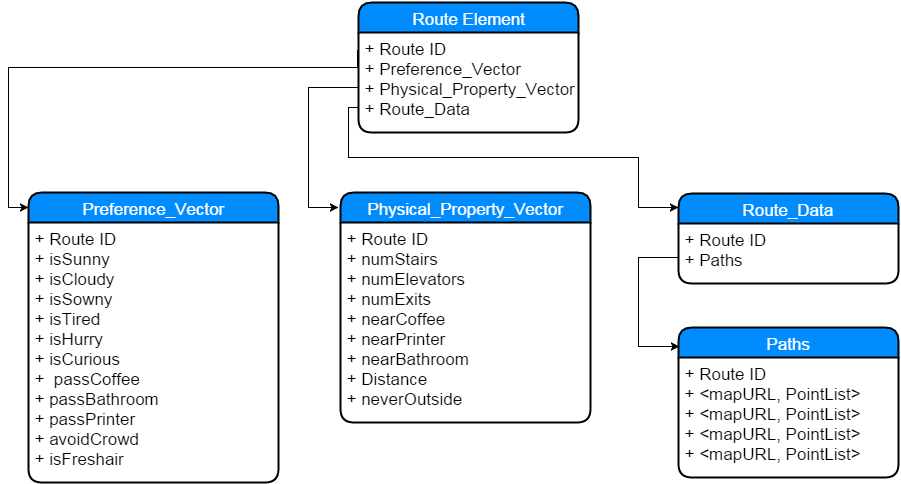
\includegraphics[width=1.0\columnwidth]{pics/element-detail.png}
\caption{Element Details}
\label{fig:element-detail}
\end{figure}

\subsection{Decision tree constructing}

A decision tree is a flowchart-like structure in which each internal node represents a \"test\" on an attribute (e.g. whether a coin flip comes up heads or tails), each branch represents the outcome of the test and each leaf node represents a class label (decision taken after computing all attributes). The paths from the root to a leaf represents classification rules.


In decision analysis, a decision tree and the closely related influence diagram are used as a visual and analytical decision support tool, where the expected values of competing alternatives are calculated.


We use Scikit-Learn, a python machine learning library, to construct these decision trees. The scikit-learn library is a powerful machine learning toolkit. Besides decision tree construction algorithms, it also provides a useful interface to generate a visual representation of the decision tree.


Using the training data we collected in the former step, we build two types of decision trees:
\begin{itemize}
\item physicalPropertyDecisionTree
\item routeSuggestionDecisionTree
\end{itemize}

\subsubsection{physicalPropertyDecisionTree}

This tree  is used to predict the desired physical properties by the users based on their current status and environment conditions. For each physical property, we build a decision tree independently. The reason we build a separate decision tree for each physical property is because we want to generate a physical property vector which doesn’t happen in the data collection step. If we build a decision tree for the entire physical property vector, all leaf nodes of the decision tree represent a vector we have met in the collection step.


\subsubsection{routeSuggestionDecisionTree}

This tree is used to predict the most suitable route according to the physical property vector. With this decision tree, given a physical properties requirement (e.g. the route should pass by a restroom), we are able to suggest a route which match the requirement as much as possible.

\subsection{Route Suggesting Procedure}
In the route suggesting procedure, the basic workflow is described in Figure~\ref{fig:route-suggest-work-flow}.

\begin{figure}[!h]
\centering
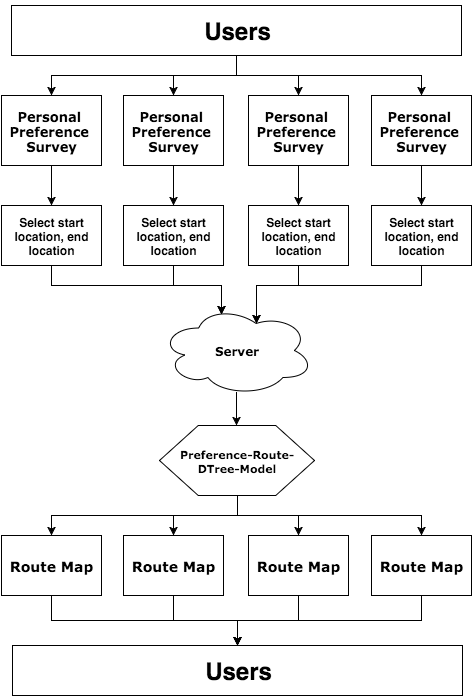
\includegraphics[width=1.0\columnwidth]{pics/route-suggest-work-flow.png}
\caption{Route Suggesting flow chart}
\label{fig:route-suggest-work-flow}
\end{figure}

The suggested route is generated based on the user’s answers to the scenario form. The generation process consists of two steps.

\subsubsection{Step 1: Physical Property Vector Generation}
The data we received from the user, which is in the same format of the survey data in modeling procedure,  is a preference vector. From the vector, we can derive the physical properties the user desires. For each property, we use the corresponding physicalPropertyDecisionTree to predict an estimated value. These values form a physical property vector.

\subsubsection{Step 2: Suggested Route Generation}
We have already generated a physical property vector in step 1. With this vector, the routeSuggestionDecisionTree can be used to generate a route suggestion.

The pseudocode for the route suggesting algorithm is:
\begin{algorithmic}\footnotesize
  \Function{routeSuggestion}{scenarioData}
    \State preferenceVector$\gets$\Call{parse}{scenarioData}
    \For{0 $\leq$ i $<$ numOfPhysicalProperties}
      \State physicalVector[i]$\gets$physicalDT[i].predict(preferenceVector) \EndFor
    \State \Return routeDT.predict(physicalVector)
  \EndFunction
\end{algorithmic}

\section{INTERFACES}
We developed a web application for users to record data for us. Our web applications have the following advantages,
\begin{itemize}
\item It is light-weighted and do not require installation. Our users can visit our system by simply opening a website in their browser.
\item It could be updated easily and quickly in the server end. Our users do not have the version problem.
\item It has high adaptability on multiply devices. Both PC users and mobile device users can reach our system easily.
\item It can be reached anytime, anywhere. Our users can label routes whenever they want. That makes it easier to collect various types of routes.
\item Collected data are highly centralized in the server and no data would be stored locally. That ensures the security and stability of data.
\end{itemize}
Our web application generally has two interfaces, record route interface and search route interface. Record Route interface allows users to fill in their personal preferences, select start location and end location and draw the route on the maps. Search Route interface allows users to fill in their personal preferences, select start location and end location and view the route plan from the server. 

\subsection{Record Route Interface}
This interface is used for recording daily routes from one room location to another across building groups. Our users need to finish the survey about their current personal preferences first, and then choose the start location and end location. After that, they can start to record the route on the webpage. The basic workflow of the record route interface is shown in Figure~\ref{fig:label-ui-flow}.

\begin{figure}[!h]
\centering
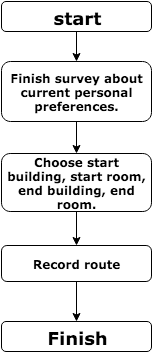
\includegraphics[width=0.4\columnwidth]{pics/label-ui-flow.png}
\caption{Workflow of Record Route Interface}
\label{fig:label-ui-flow}
\end{figure}

Users will first be presented the personal preferences page, as shown in Figure~\ref{fig:personal_page}, and finish the preference survey. At the bottom of this page, there is a \"Go record\" button. After finishing the survey, users will click the button. Then users will be navigated to the route drawing page, as shown in Figure~\ref{fig:routedraw_page}.

\begin{figure}[!h]
\centering
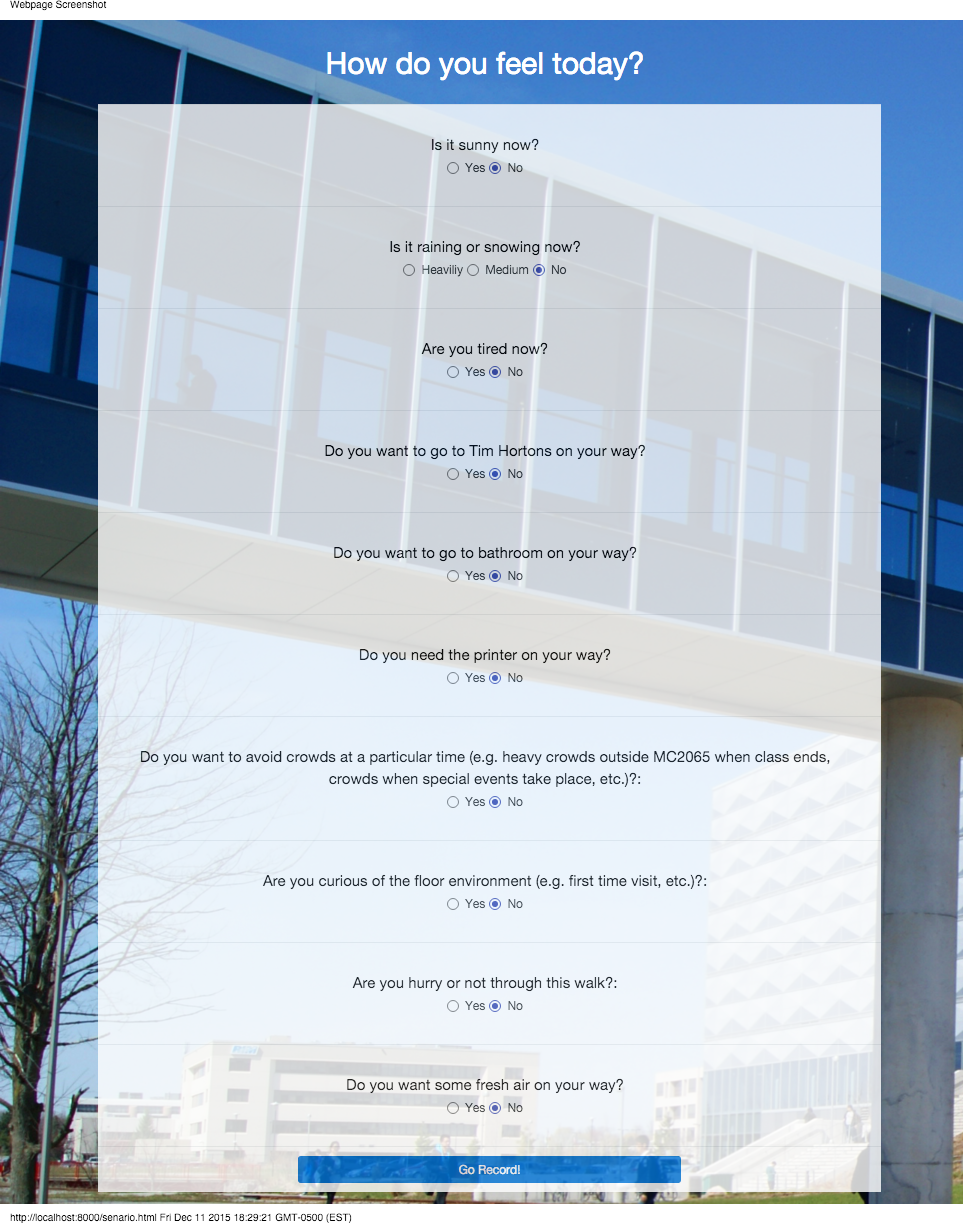
\includegraphics[width=1.0\columnwidth]{pics/personal_page.png}
\caption{Personal Preference Page}
\label{fig:personal_page}
\end{figure}

\begin{figure}[!h]
\centering
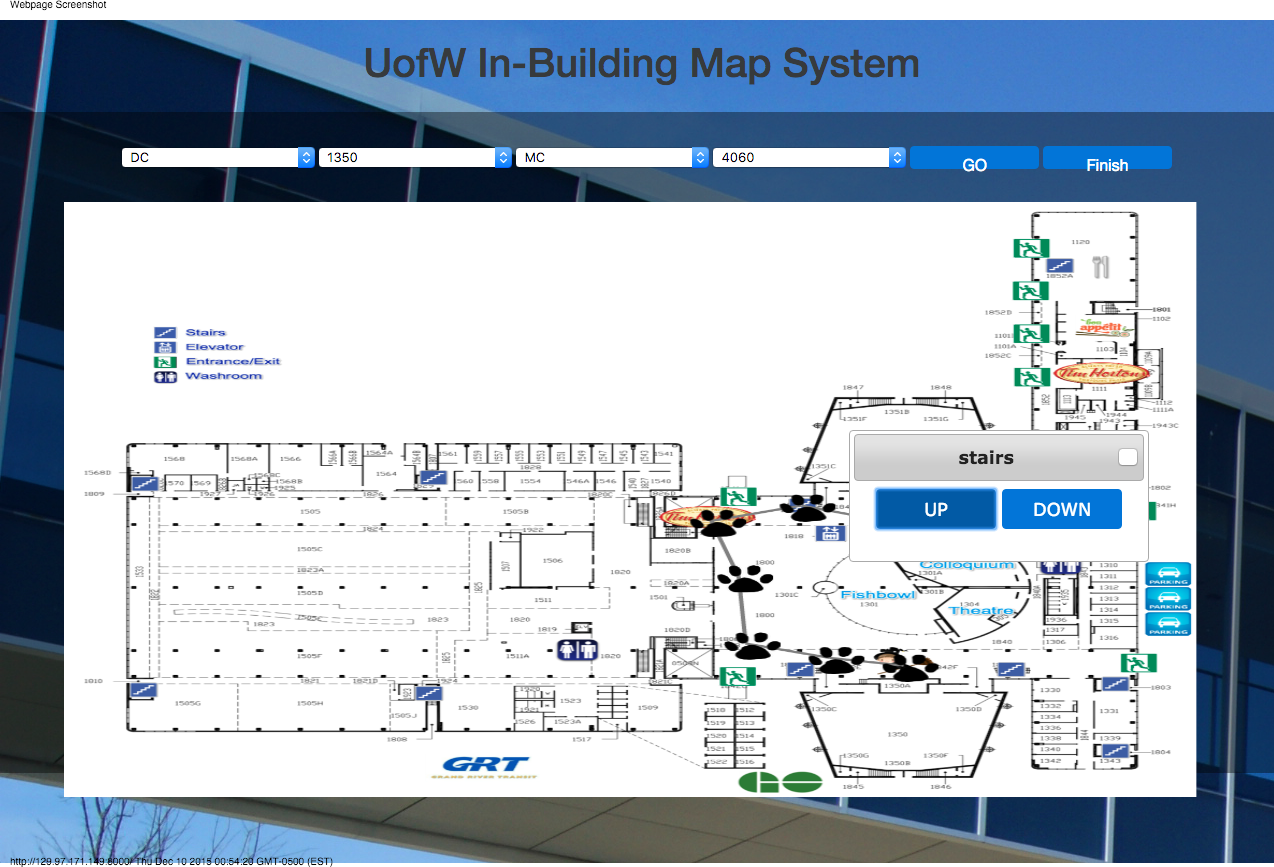
\includegraphics[width=1.0\columnwidth]{pics/routedraw_page.png}
\caption{Welcome Page}
\label{fig:routedraw_page}
\end{figure}

Users will choose their start building, start room, end building, end room from the top menus on the page, as shown in Figure~\ref{fig:choose_page}, and click \"GO\" button on the right side of the menu.


\begin{figure}[!h]
\centering
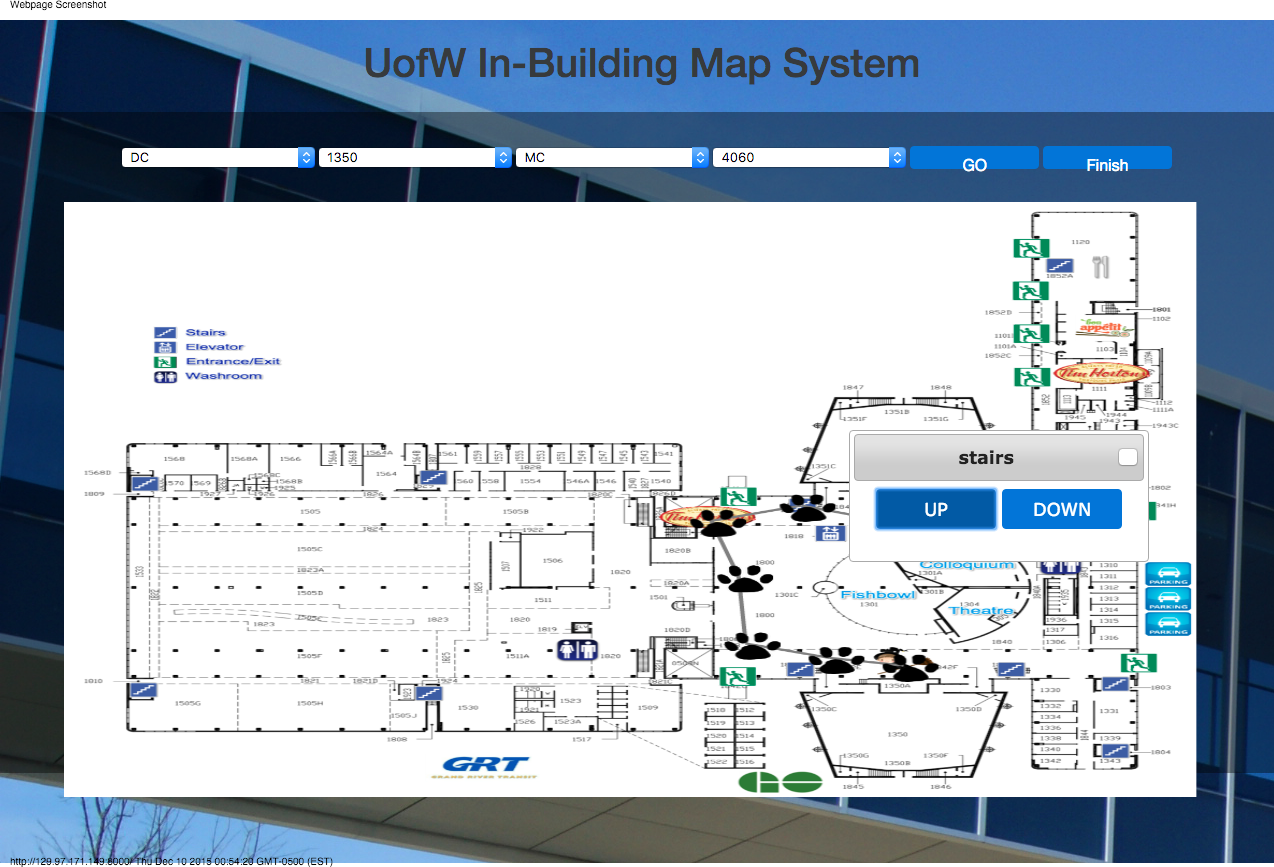
\includegraphics[width=1.0\columnwidth]{pics/choose_page.png}
\caption{Choose Page}
\label{fig:choose_page}
\end{figure}


Once the \"GO\" button is clicked, the user will be presented the floor map of the start location he chose, a little wizard riding a broom is placed on the map indicating the location of the start room, as shown in Figure~\ref{fig:map0}. There are many labels on the map (e.g. bathroom labels, the Tim Hortons labels, bus stop labels, printer labels) to help users to picture the environment in their brains better. 

\begin{figure}[!h]
\centering
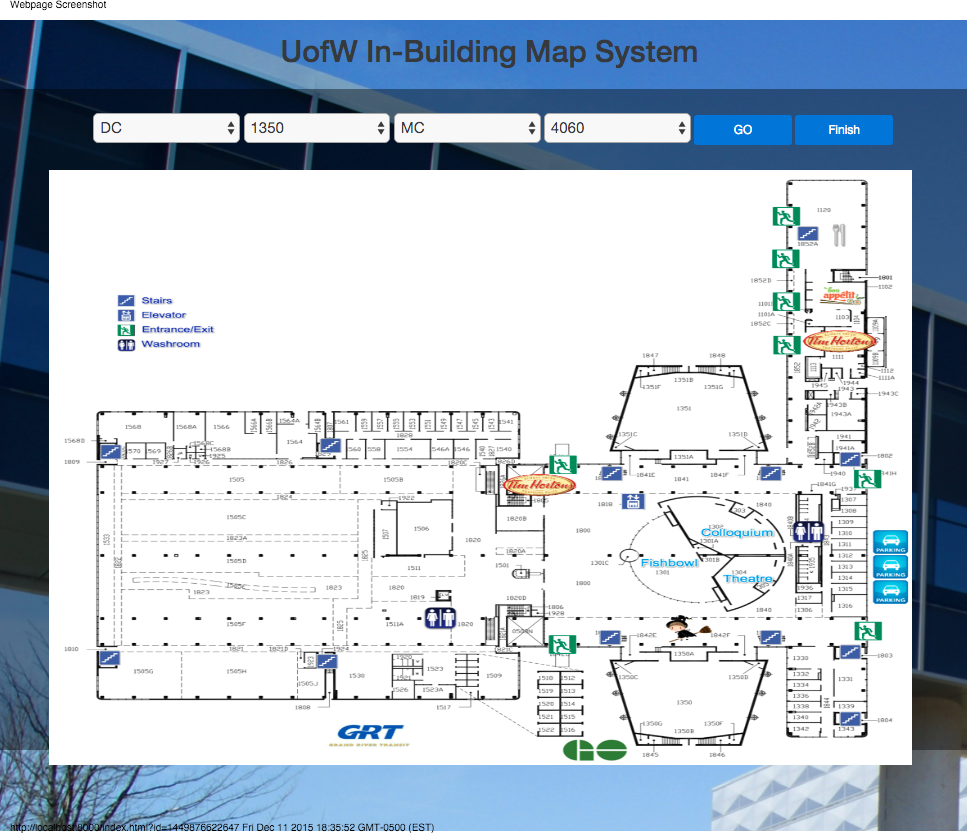
\includegraphics[width=1.0\columnwidth]{pics/map0.png}
\caption{Start view}
\label{fig:map0}
\end{figure}

Users can start drawing their routes by simply clicking on the map. Their first step shall be the start room. Each time they clicked, a footprintwill be drawn on the map. Neighboring steps will have connected footprints, as shown in Figure~\ref{fig:map1}.

\begin{figure}[!h]
\centering
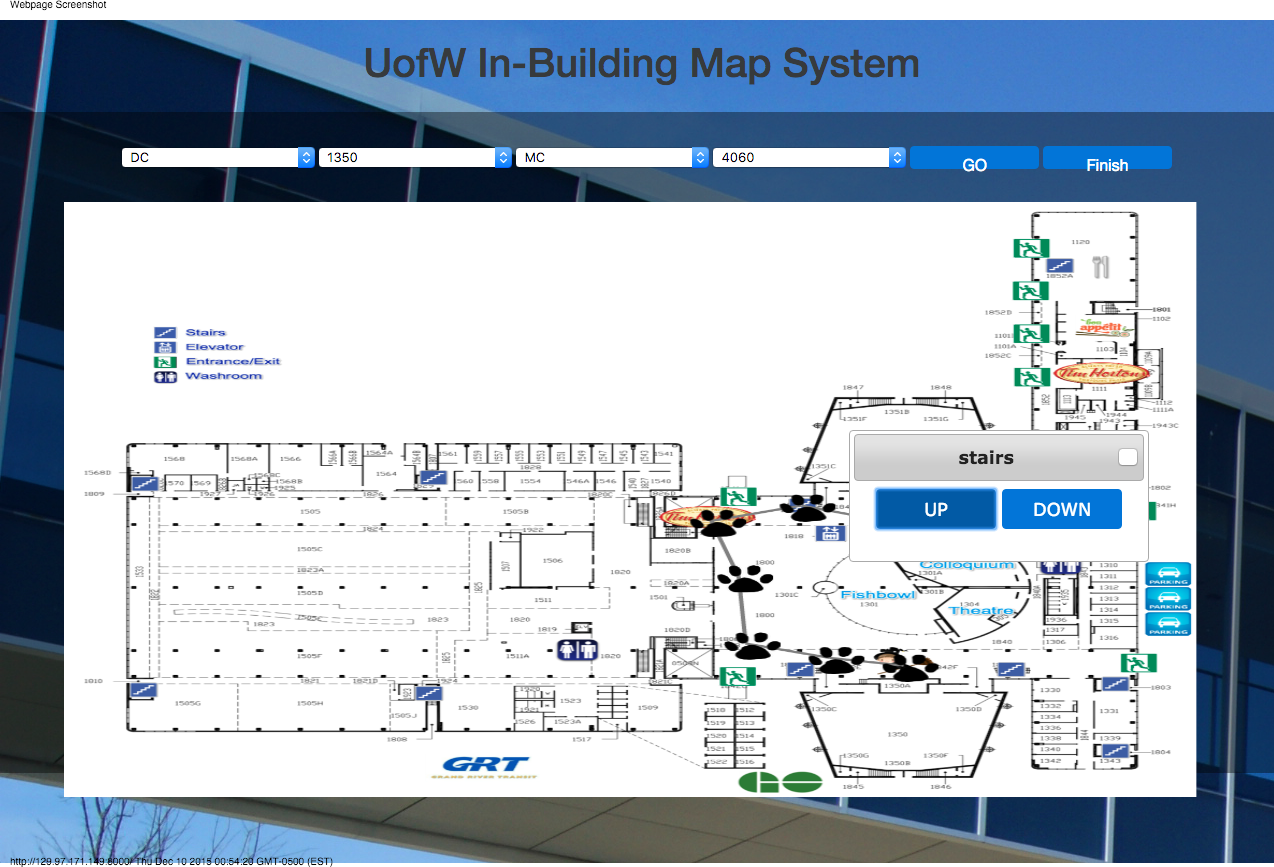
\includegraphics[width=1.0\columnwidth]{pics/map1.png}
\caption{Footprints on the map}
\label{fig:map1}
\end{figure}


Stairs and elevators are also labeled on the maps. If our users need to go up stairs or down stairs, they can click the stairs or the elevators on the map. A popup dialog will be presented when those labels are clicked. Users can choose to go up, down or just close the dialog in the dialog, as shown in Figure~\ref{fig:map2}.

\begin{figure}[!h]
\centering
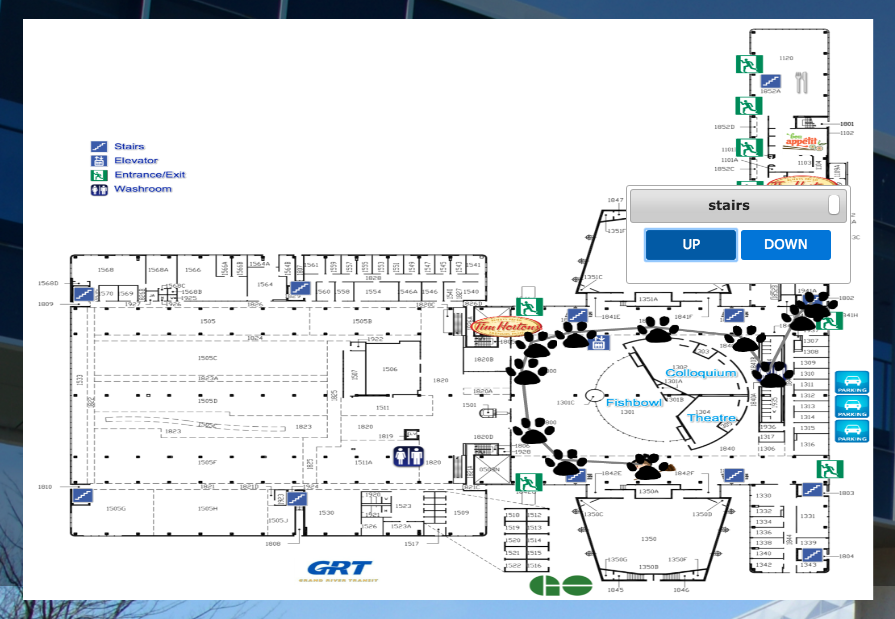
\includegraphics[width=1.0\columnwidth]{pics/map2.png}
\caption{Clicked stairs or elevators on the map}
\label{fig:map2}
\end{figure}

The corresponding floor map will be presented on the webpage if the users clicked going up or going down. Floor maps in the same building are aligned and in the same scale. Therefore, users can easily find out the stairs or the elevator they come from. Users can keep drawing routes on the new floor map by clicking on the map, as shown in Figure~\ref{fig:map3}.

\begin{figure}[!h]
\centering
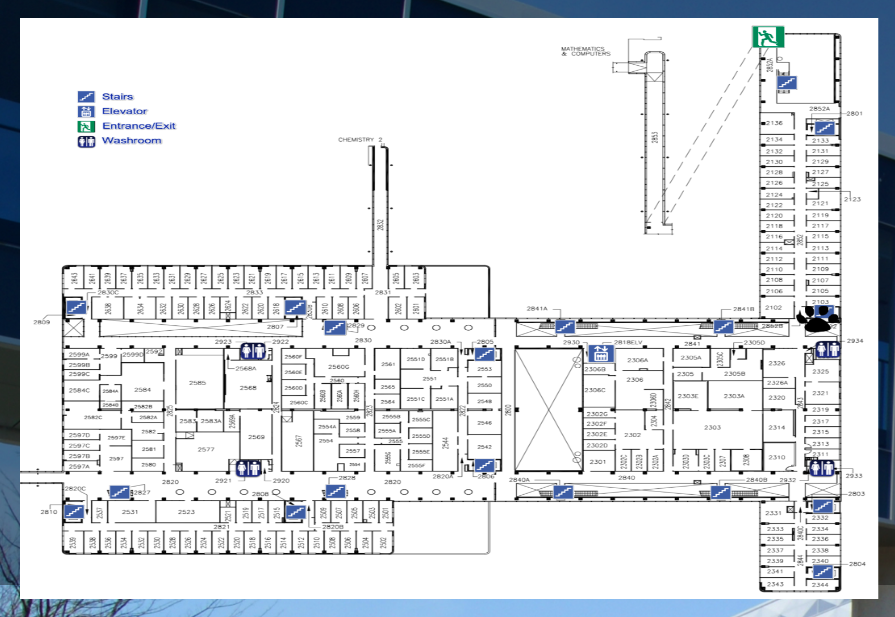
\includegraphics[width=1.0\columnwidth]{pics/map3.png}
\caption{New map after going up or down stairs}
\label{fig:map3}
\end{figure}

Exits and entrances are labeled on the maps as well. If our users need to exit the building, they can click the exit on the map. The same as above, a popup dialog will be presented and users can choose to exit the building, enter the building or just close the dialog in the dialog, as shown in Figure~\ref{fig:map4}.


\begin{figure}[!h]
\centering
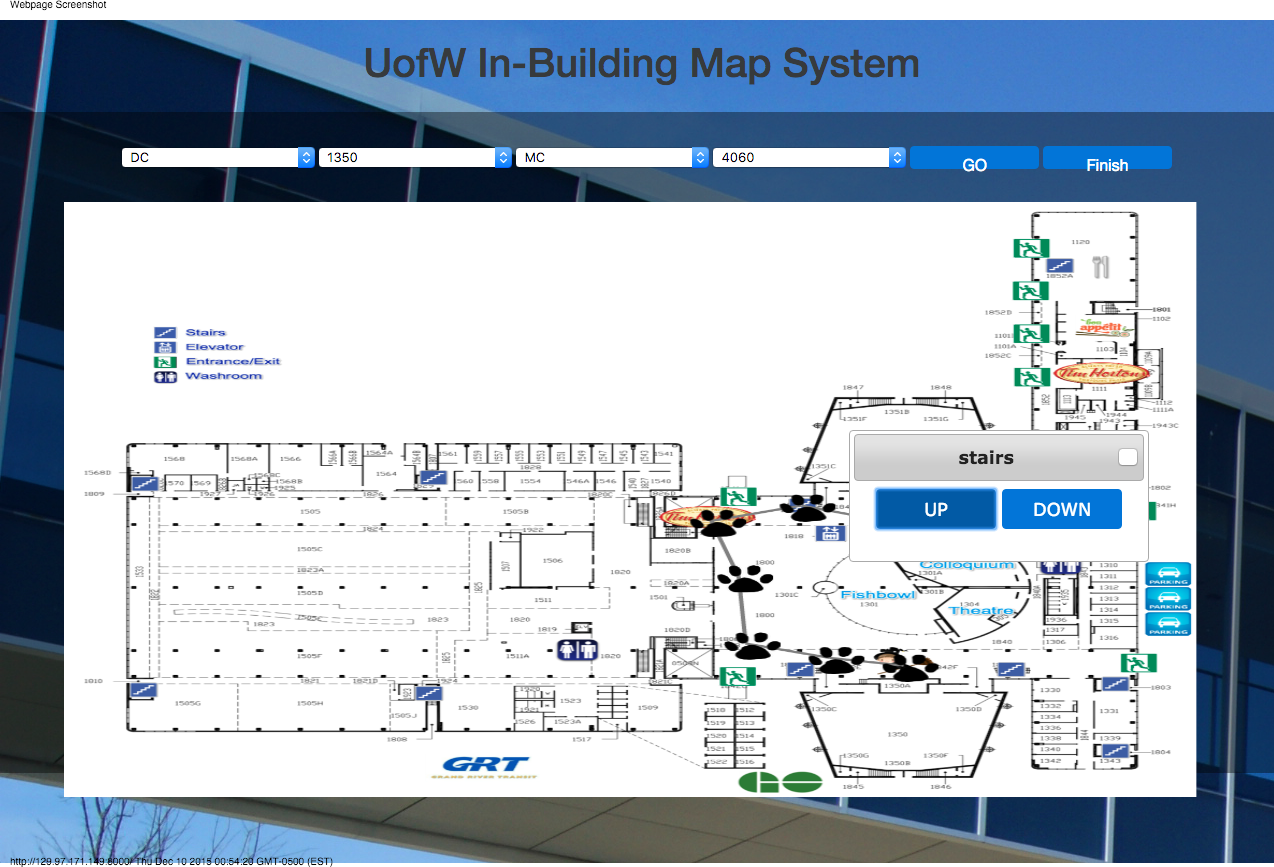
\includegraphics[width=1.0\columnwidth]{pics/map4.png}
\caption{Clicked exirts or entrances on the map}
\label{fig:map4}
\end{figure}

So far, our system supports MC building and DC building. Therefore, we already calculated which floor in which building users can get after exiting each of the exits (e.g. users will get the third floor of MC building after exiting the exit on the second floor of DC building). When the users click the exit button on the dialog, they will be presented the corresponding floor map of the expected floor in the expected building. Users can adjust the floor by simply click the stairs labels if they found they are not on their expected floors. When presented the expected floor, users will need to specify the entrance they use to enter the building by click on the entrance label on the map and choose \"enter\" on the popup dialog. Once they entered the building, they can continue to draw maps as before, as shown in Figure~\ref{fig:map5}.


\begin{figure}[!h]
\centering
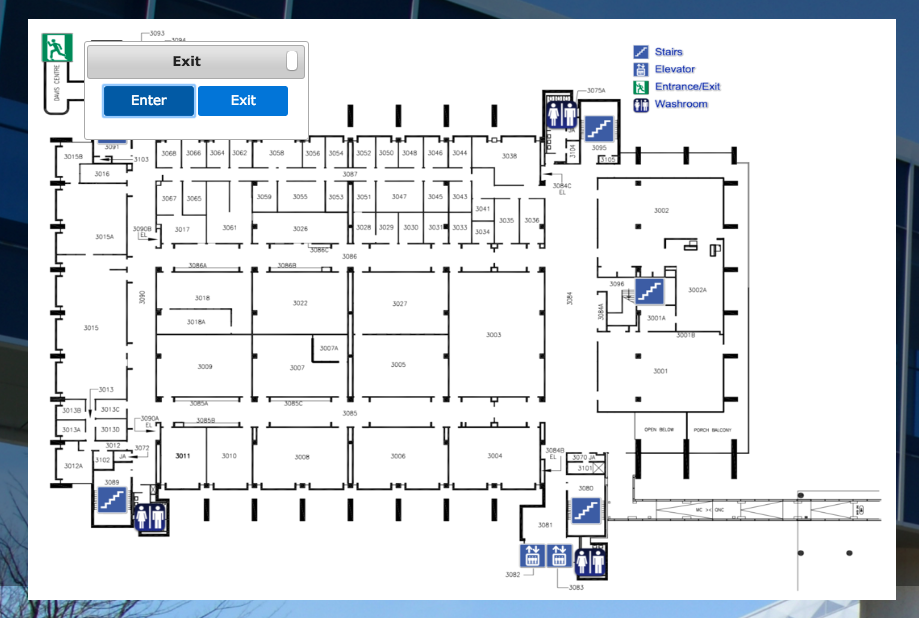
\includegraphics[width=1.0\columnwidth]{pics/map5.png}
\caption{New map after exiting a building}
\label{fig:map5}
\end{figure}

After the users arrived their destination, they will click the finish button on the right side of menus. Once the finish button is clicked, the route is recorded in the server and the users will be presented a thank you on the webpage, as shown in Figure~\ref{fig:map6} and Figure~\ref{fig:map61}.

\begin{figure}[!h]
\centering
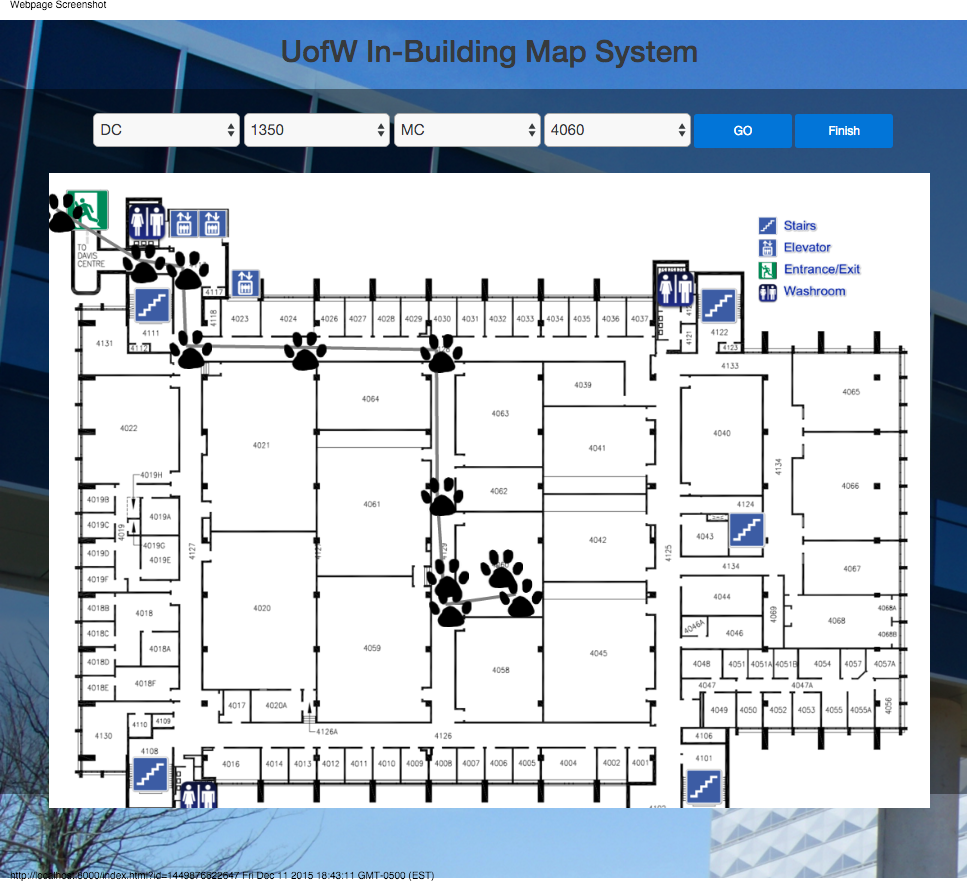
\includegraphics[width=1.0\columnwidth]{pics/map6.png}
\caption{Arriving destination}
\label{fig:map6}
\end{figure}

\begin{figure}[!h]
\centering
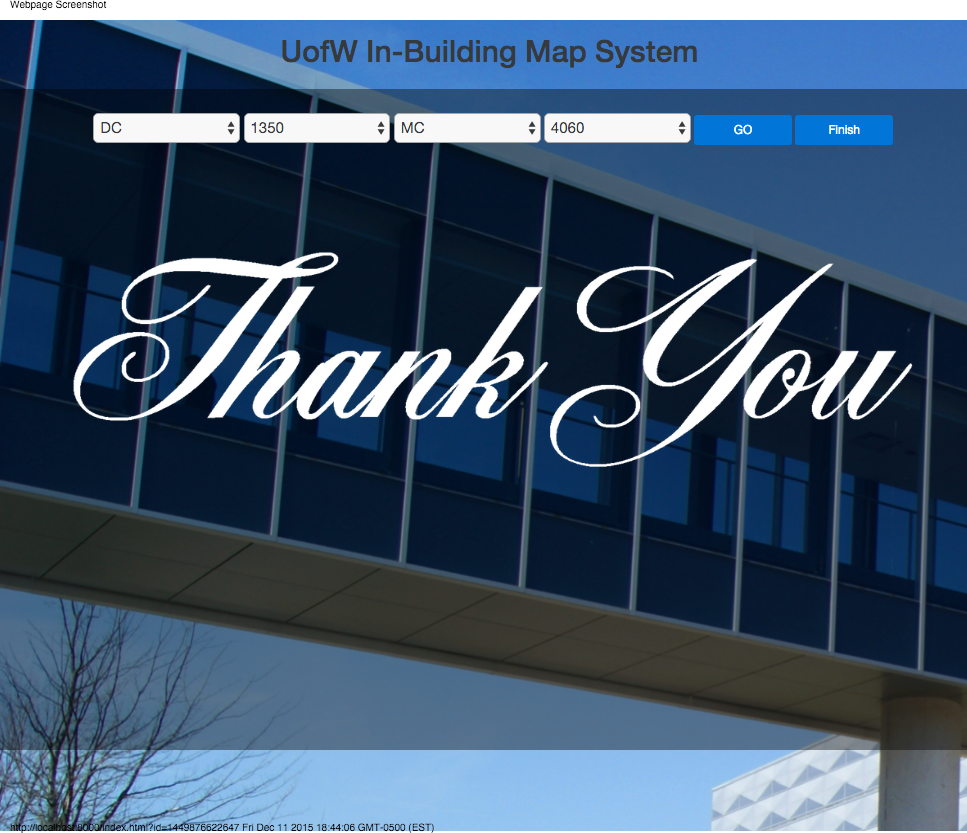
\includegraphics[width=1.0\columnwidth]{pics/map61.png}
\caption{Thank you page}
\label{fig:map61}
\end{figure}

\subsection{Seachroute Interface}
This interface is used for search routes from one room location to another across building groups with personal preferences. Our users need to finish the survey about their current personal preferences first, and then choose the start location and end location. After that, the route will be presented on the webpage. The basic workflow of the record route interface is shown in Figure~\ref{fig:find-uiflow}.

\begin{figure}[!h]
\centering
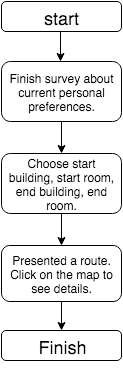
\includegraphics[width=0.4\columnwidth]{pics/find-uiflow.png}
\caption{Workflow of Seachroute Interface}
\label{fig:find-uiflow}
\end{figure}


Same as above, users will first be presented the personal preferences page, as shown in Figure~\ref{fig:personal_page_1}, and finish the preference survey. At the bottom of this page, there is a \"Find route!\" button. After finishing the survey, users will click the button. Then users will be nevigated to the route presenting page.

\begin{figure}[!h]
\centering
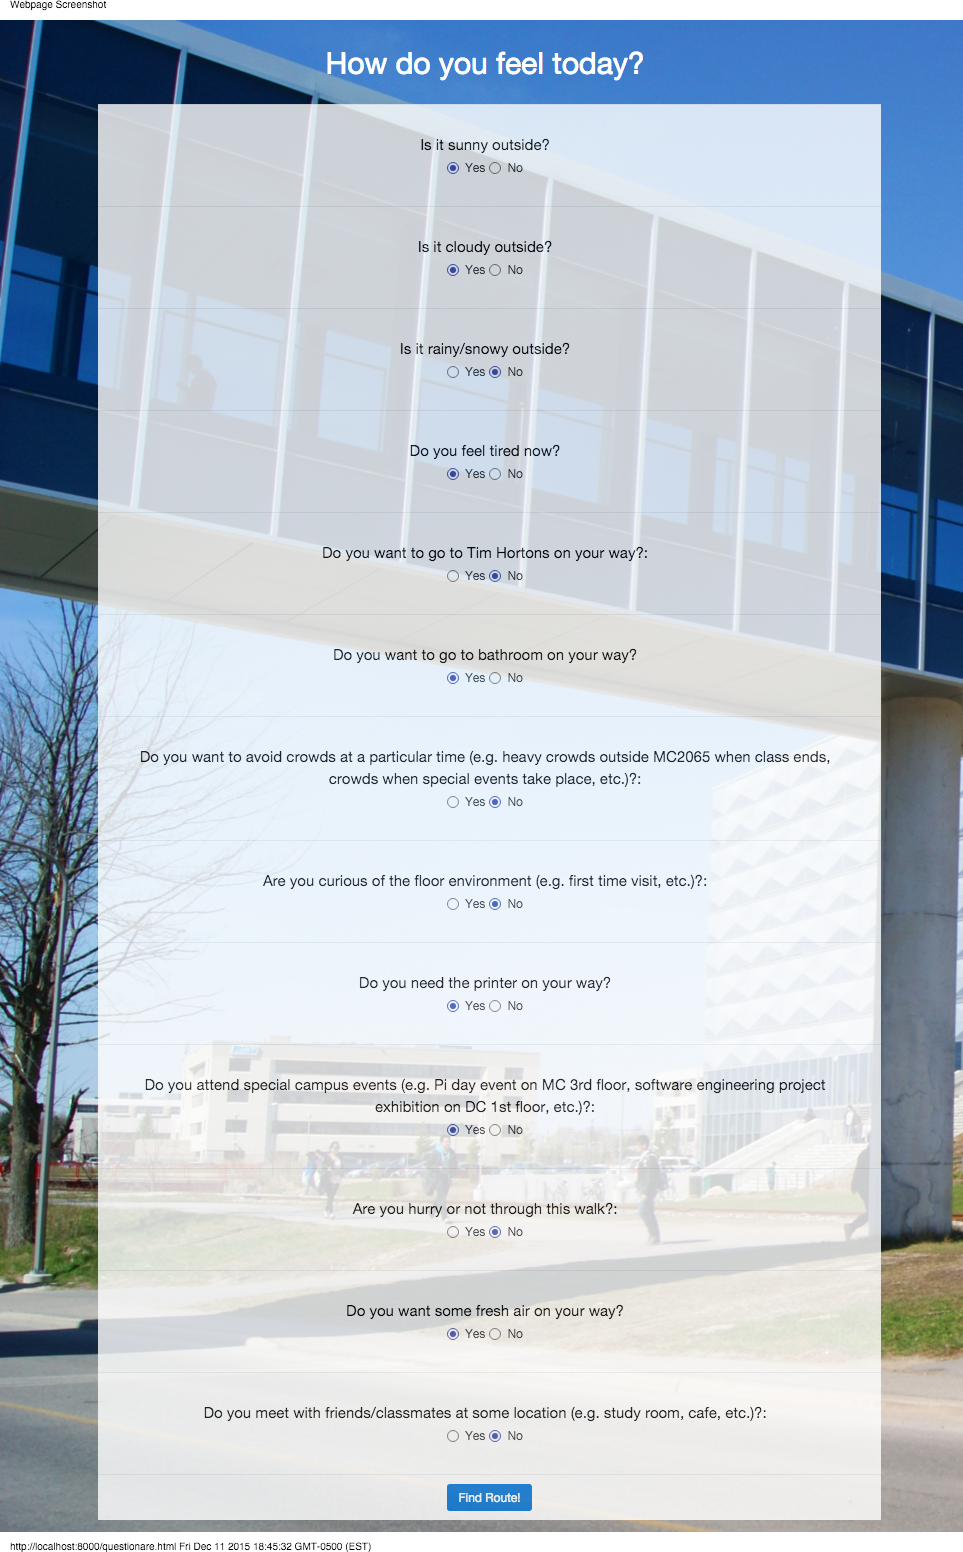
\includegraphics[width=1.0\columnwidth]{pics/personal_page_1.png}
\label{fig:personal_page_1}
\caption{Personal preferences page of Search Route Interface}
\end{figure}


Users will choose their start building, start room, end building, end room from the top menus on the page, as shown in Figure~\ref{fig:choose_page_1}, and click \"Find\" button on the right side of the menu.

\begin{figure}[!h]
\centering
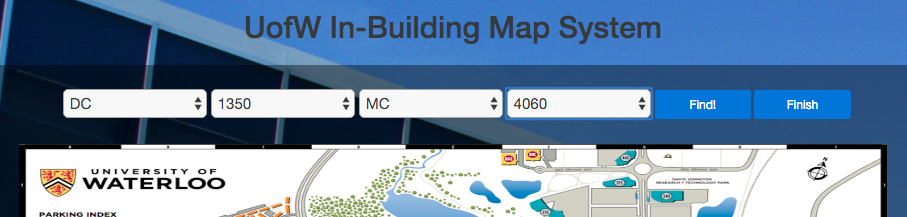
\includegraphics[width=1.0\columnwidth]{pics/choose_page_1.png}
\caption{Choose start location and end location}
\label{fig:choose_page_1}
\end{figure}

Once the \"GO\" button is clicked, the webpage will send the server the request and the server will reply the webpage with the proper route. Then the user will be presented the floor map of the start location he chose, with connected footprints on it, as shown in Figure~\ref{fig:map7}. There are also many labels on the map (e.g. bathroom labels, the Tim Hortons labels, bus stop labels, printer labels) to help users to picture the environment in their brains better. 

\begin{figure}[!h]
\centering
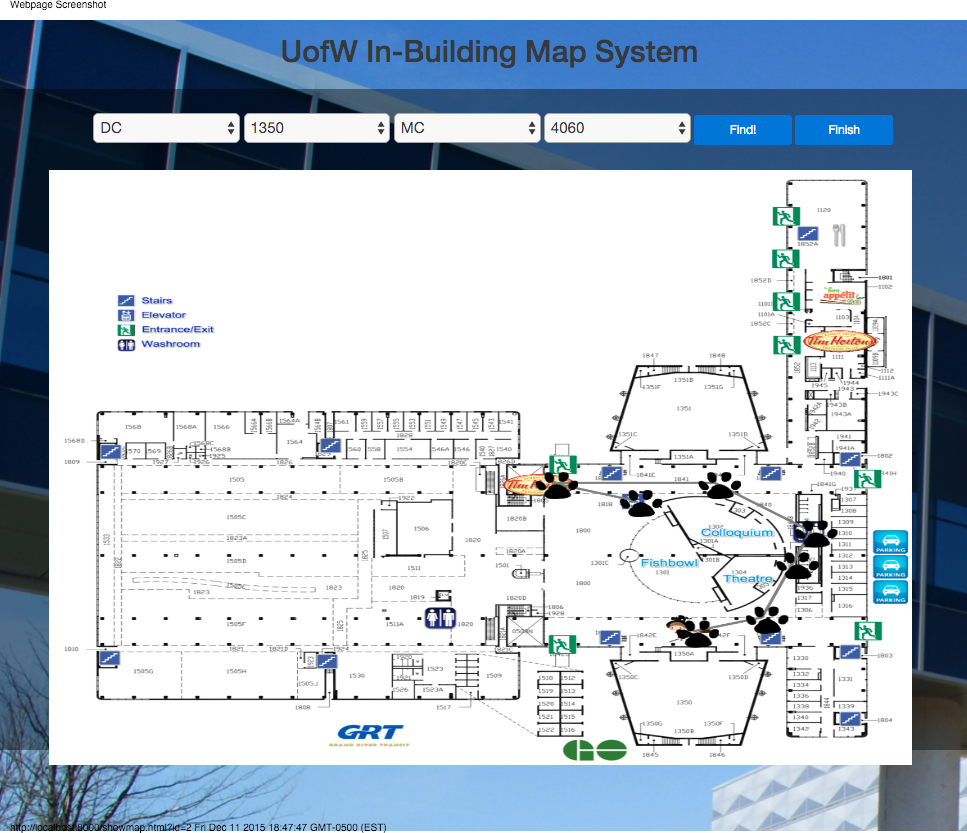
\includegraphics[width=1.0\columnwidth]{pics/map7.png}
\caption{Map with proper route}
\label{fig:map7}
\end{figure}

Our users will follow those footprints on the map. If the footprints on the current floor map end up on a stairs label or elevator label, the users can click on that label and a popup dialog will be presented, as shown in Figure~\ref{fig:map8}. Users can choose to go up or down stairs in the dialog. However, this time, only the correct direction will be responded. That is to say, if the planned route goes upstairs from the second floor of DC to the first floor of DC, the map will not change if users click going upstairs on the second floor.

\begin{figure}[!h]
\centering
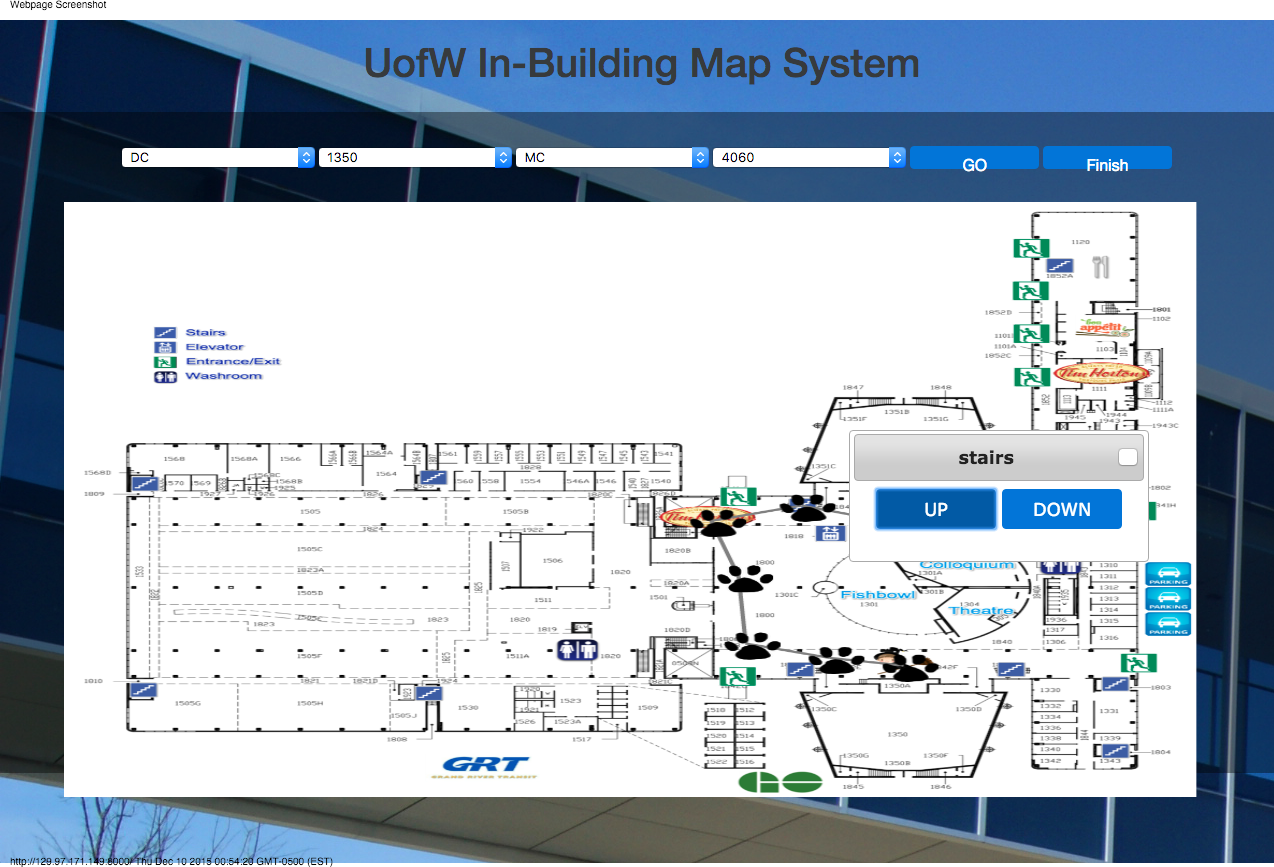
\includegraphics[width=1.0\columnwidth]{pics/map8.png}
\caption{Clicked stairs on the map}
\label{fig:map8}
\end{figure}


If it is the correct direction of stairs or elevators, the corresponding floor map as well as the footprints will be presented, as shown in Figure~\ref{fig:map9}.

\begin{figure}[!h]
\centering
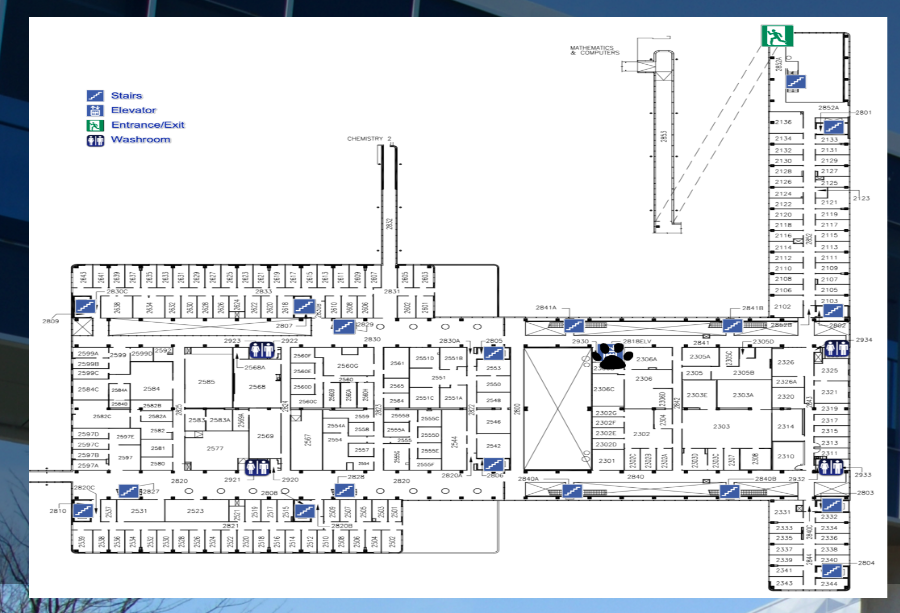
\includegraphics[width=1.0\columnwidth]{pics/map9.png}
\caption{Corresponding map shown after going up or down}
\label{fig:map9}
\end{figure}

The same rules apply on exits and entrances as well, as shown in Figure~\ref{fig:map10} and Figure~\ref{fig:map11}.

\begin{figure}[!h]
\centering
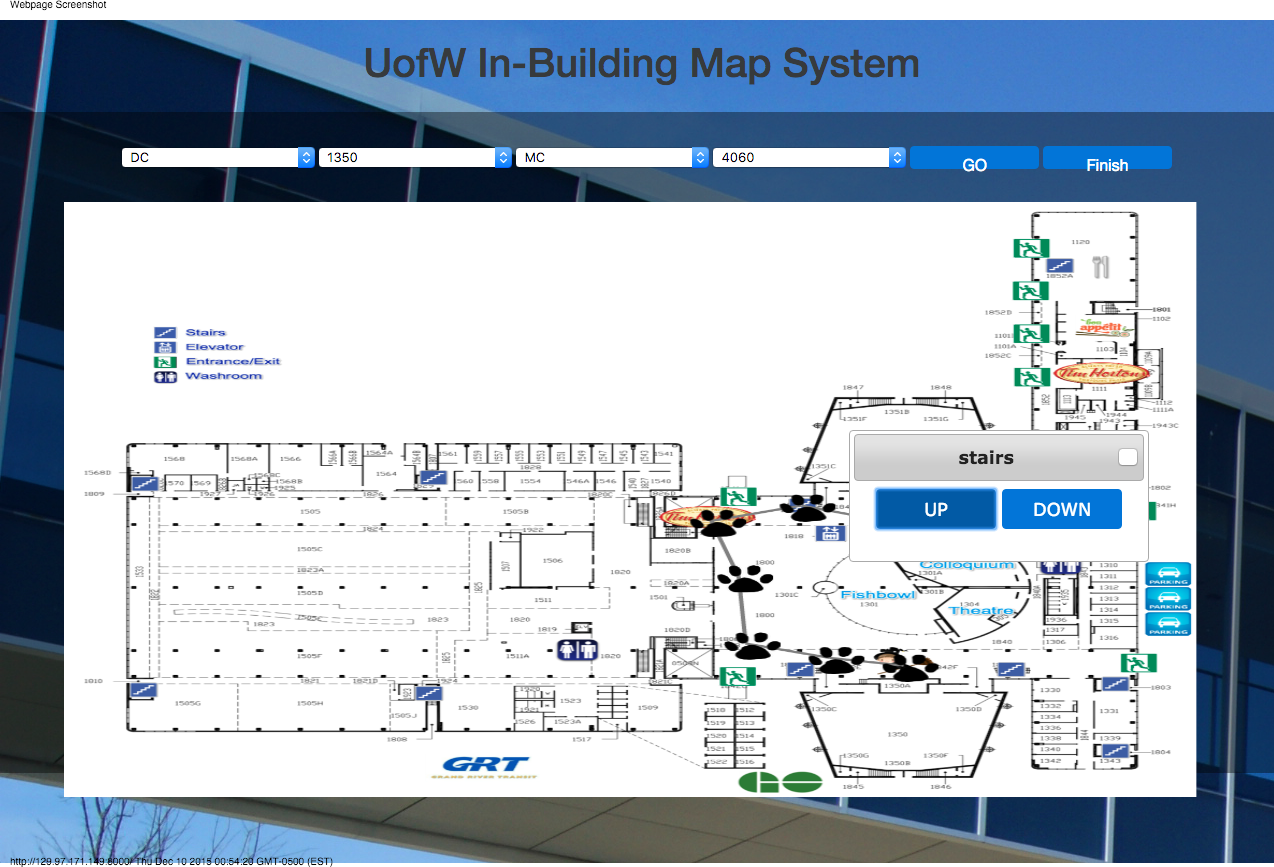
\includegraphics[width=1.0\columnwidth]{pics/map10.png}
\caption{Clicked exits on the map}
\label{fig:map10}
\end{figure}

\begin{figure}[!h]
\centering
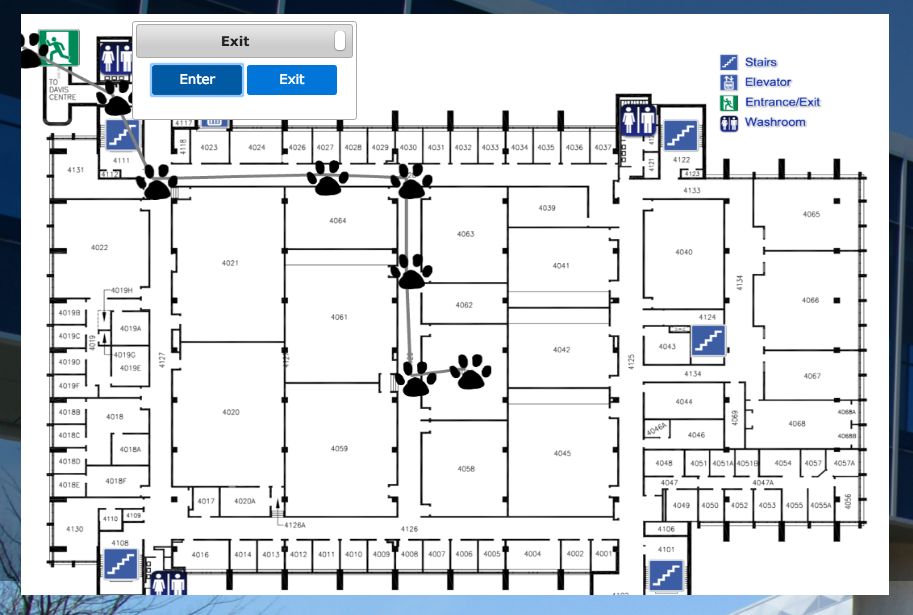
\includegraphics[width=1.0\columnwidth]{pics/map11.png}
\caption{Clicked entrances on the map}
\label{fig:map11}
\end{figure}

\section{EXPERIMENT}

In this section, we explain how we execute the crowdsourcing to collect data for training the model based on decision tree algorithms.

\subsection{Experiment Setup}
\subsubsection{Participants}
Since drawing a route between two specific rooms in the campus of the University of Waterloo requires a relatively high degree of familiarity of the campus. Thus, the participants are UW students. 48 students in total participated in our experiment. These students have been UW for at least 2 months.
\subsubsection{ Source and Destination}
To simplify our experiment, currently, we only support routes from DC 1350 to MC 4060. All of the participants are familiar with these two buildings. Since the number of participants is limited, supporting more source and destination pairs may reduce the data for each pair.

\subsection{Experiment Methodology}

The experiment consists of two steps:


Step 1: Take a survey about the current status of the participant and the environment conditions. All participants are asked to answer all questions listed in table-XX (see modeling procedure). All these data is sent to the server and associated with a route ID.


Step 2: Draw a route from DC 1350 to MC 4060. The users are asked to plan the route according to their answers to the survey taken in step 1. The coordinates of points the user click on the map will be sent to the server as the route data. The route data is also associated with the route ID in step 1.


After these two steps, all data collection work has been finished. In summary, for each user, the data we collect includes:
\begin{itemize}
\item Survey answers
\item Routes data
\end{itemize}

Step 3: Derive physical properties from the data of each route. PhysicalPropertyDecisionTrees are generated based on the physical properties and survey answers. RouteSuggestionDecisionTree is generated based on the physical properties and route data.

\section{RESULT}

In our experiment, we generate 8 decision trees. 7 of them are for predicting physical properties based on a preference vector. The other one left is for predicting the route number based on a physical property vector.

Figure ~\ref{fig:dt1} shows the decision tree for predicting the number of stairs the route should use based on the user’s preference. 

Figure ~\ref{fig:dt2} shows the decision tree for predicting how many levels of elevators the route should use. 

Figure ~\ref{fig:dt3} shows the decision tree for predicting how many exits the route should pass. 

Figure ~\ref{fig:dt4} shows the decision tree for predicting if the route should pass by a coffee shop. 

Figure ~\ref{fig:dt6} shows the decision tree for predicting if the route should pass by a rest room. 

Figure ~\ref{fig:dt7} shows the decision tree for predicting how long if the route. 

Figure ~\ref{fig:dt8} shows the decision tree for predicting if the route goes outside the building.


Figure ~\ref{fig:dt9} shows the decision tree for predicting which route should be picked.


There are several clarifications about the graph.
\begin{itemize}
\item For each non-leaf node of a decision tree, the first line is the condition to be checked. 
\item The gini value of each node is positive correlative to the probability of the wrong prediction. A large gini value suggests the probability of wrong prediction is high.
\item The value of samples means how much samples are left after following all the path from the root to the current node.
\item Each element in the value array means the number of samples of the corresponding class.
\item The value of class means the prediction value. This value is only shown in the routeSuggestionDecisionTree.
\end{itemize}

The physical properties are predicted by the decition trees in Figure~\ref{figdt1} to Figure~\ref{fig:dt8}. As we can see from the graphs, 49 out of 64 leaf nodes in physical property decision trees has the gini factor of 0.0. That indicates a relatively high accuricy in physical property predicting. 


The final route is selected by the decision tree in Figure~\ref{fig:dt9}. The gini factor in this decision tree is relatively higher that thoses in physical property decision trees. The possible reason is that this decision tree is used to predict which route to choose given a set of personal prefrences, for one set of personal preferences, there may exit more than one routes that satisfies those preferences. For example, the leaf node on the right of the red bottom leaf node, has 9 possible routes that satisfy the given preferences set. Thoses 9 routes should all be presented to the users. 


\begin{figure*}[!h]
\centering
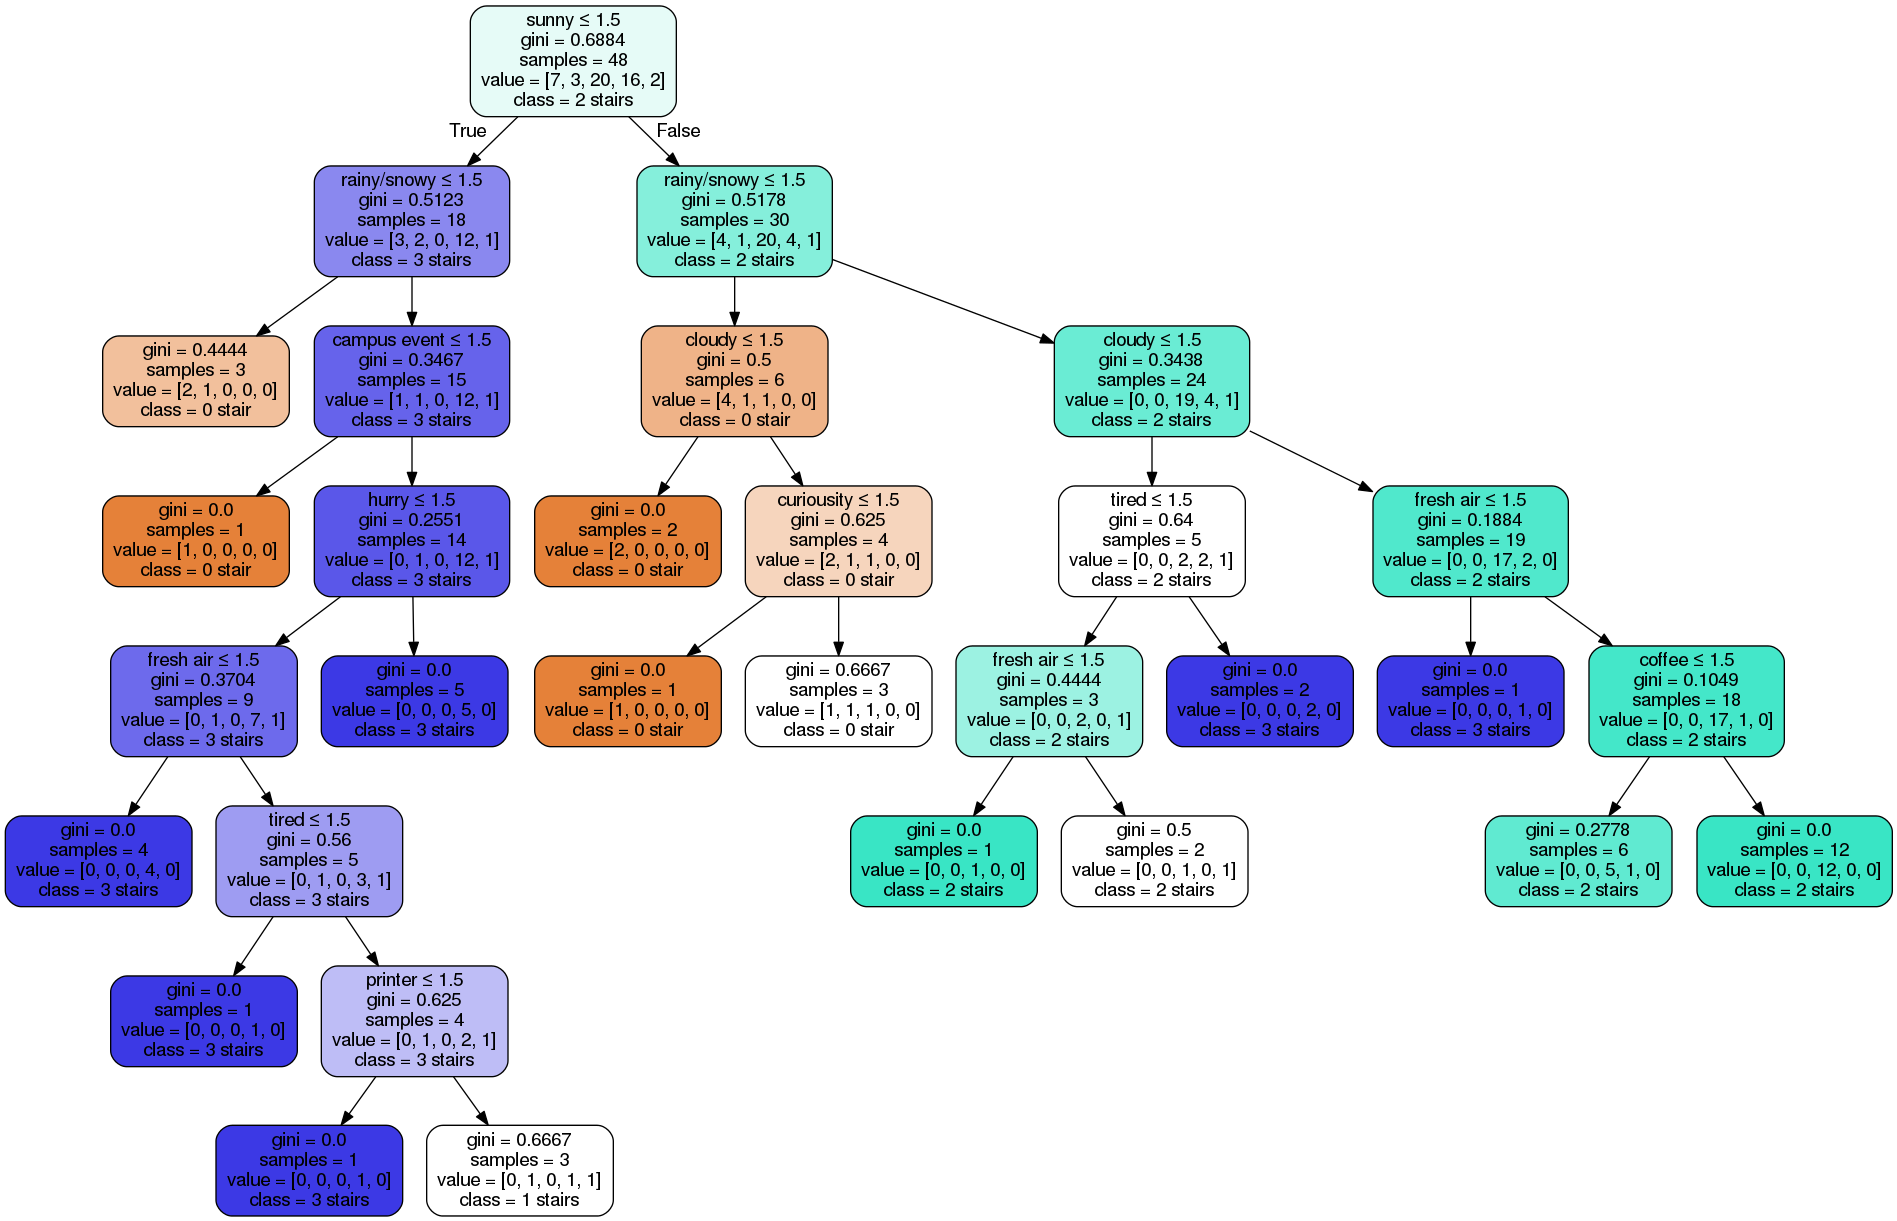
\includegraphics[width=2.0\columnwidth]{pics/decisionTree_1.png}
\caption{Decision tree for predicting the number of stairs the route should use based on the user’s preference.}
\label{fig:dt1}
\end{figure*}

\begin{figure*}[!h]
\centering
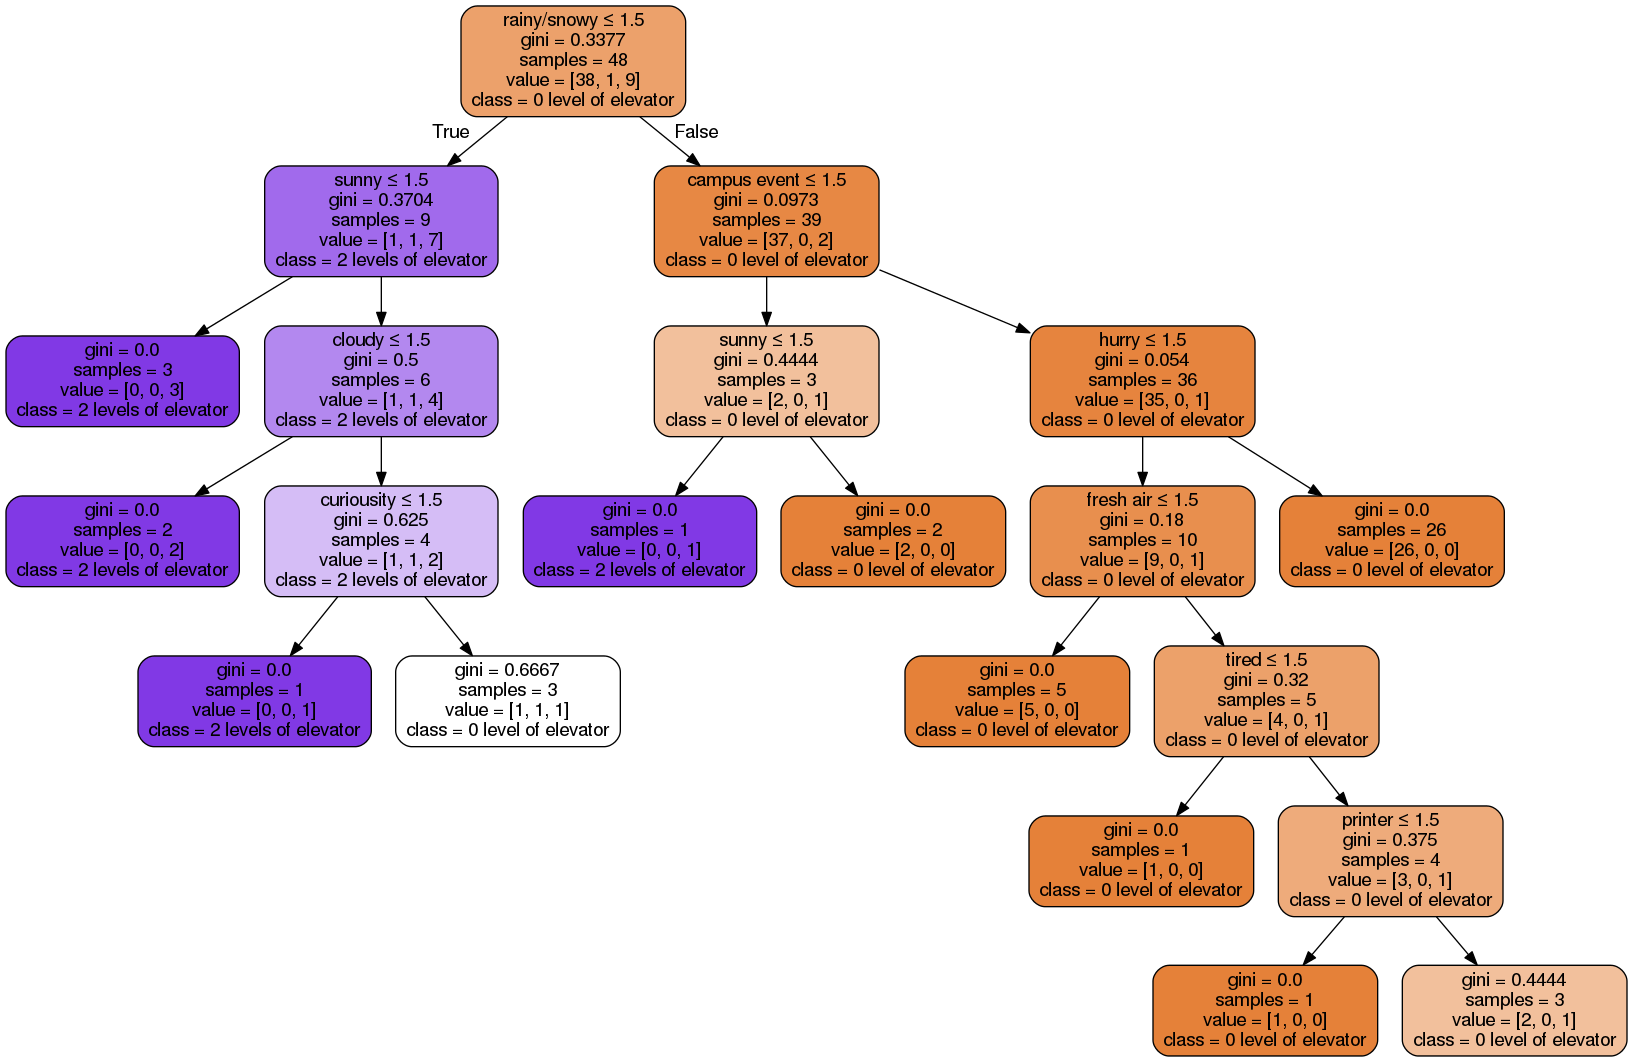
\includegraphics[width=2.0\columnwidth]{pics/decisionTree_2.png}
\caption{Decision tree for predicting how many levels of elevators the route should use.}
\label{fig:dt2}
\end{figure*}

\begin{figure*}[!h]
\centering
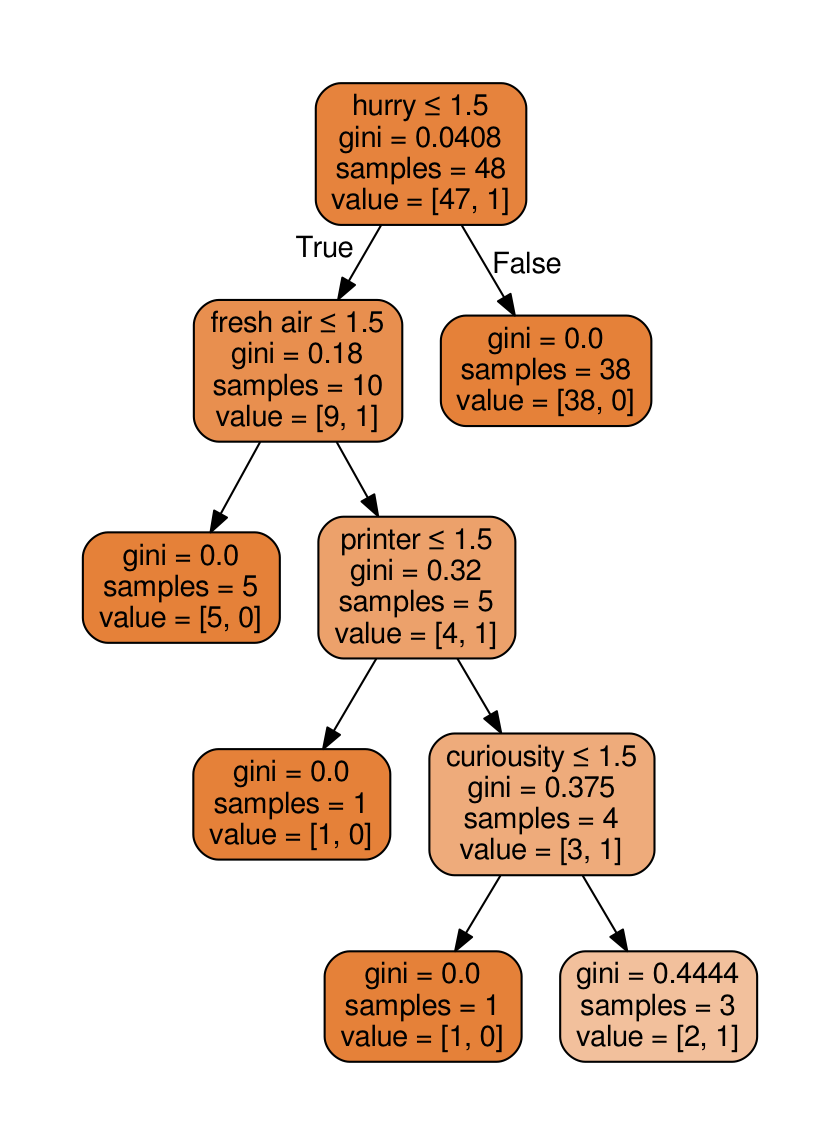
\includegraphics[width=0.7\columnwidth]{pics/decisionTree_3.png}
\caption{Decision tree for predicting how many exits the route should pass.}
\label{fig:dt3}
\end{figure*}

\begin{figure*}[!h]
\centering
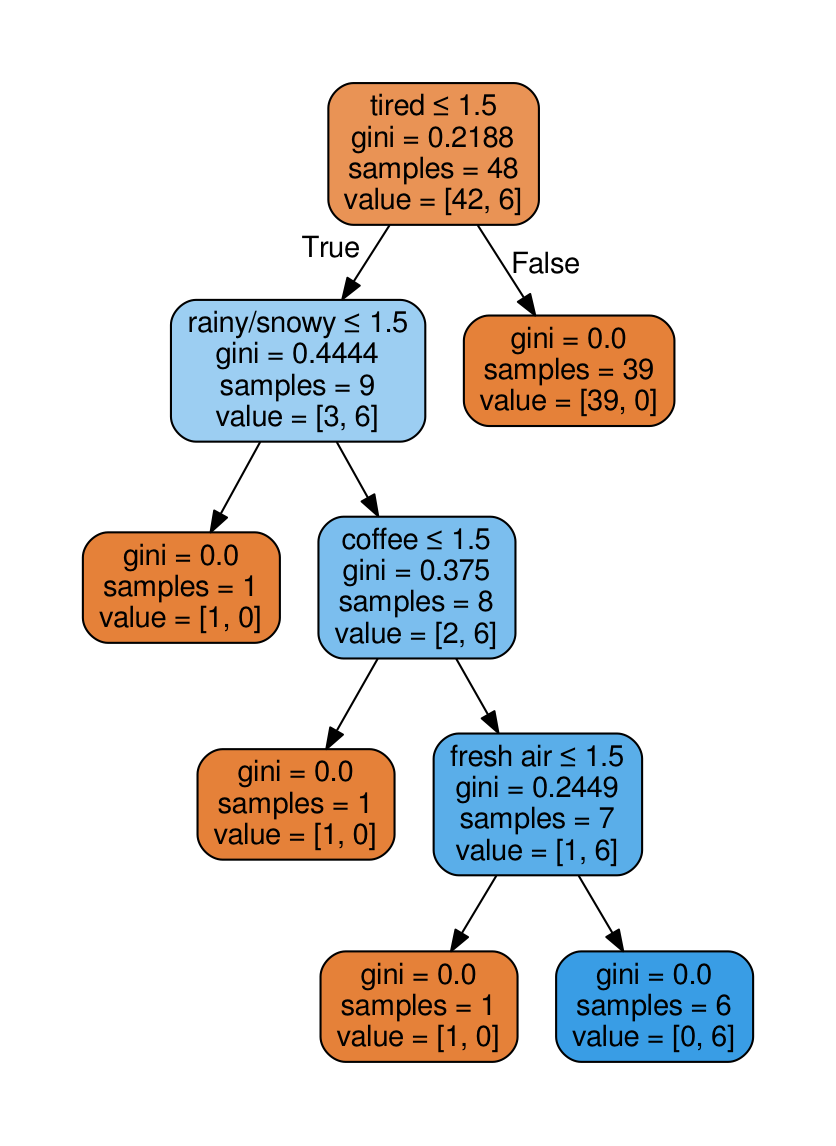
\includegraphics[width=0.7\columnwidth]{pics/decisionTree_4.png}
\caption{Decision tree for predicting if the route should pass by a coffee shop.}
\label{fig:dt4}
\end{figure*}

\begin{figure*}[!h]
\centering
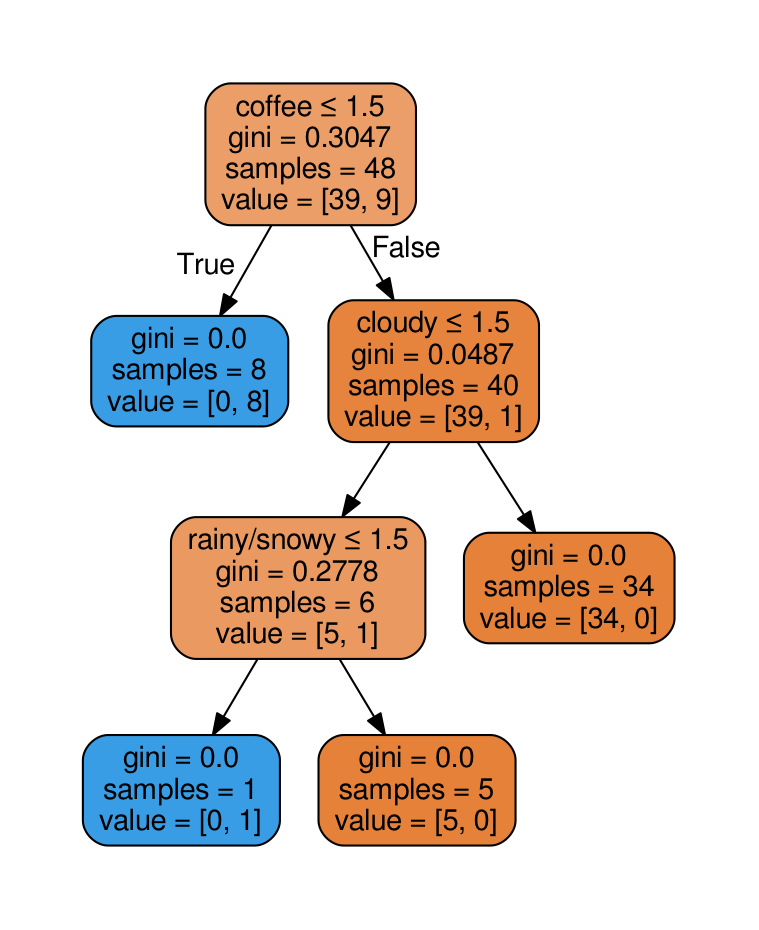
\includegraphics[width=0.7\columnwidth]{pics/decisionTree_6.png}
\caption{Decision tree for predicting if the route should pass by a rest room..}
\label{fig:dt6}
\end{figure*}

\begin{figure*}[!h]
\centering

\includegraphics[width=2.0\columnwidth]{pics/decisionTree_7.png}
\caption{Decision tree for predicting how long if the route.}
\label{fig:dt7}
\end{figure*}

\begin{figure*}[!h]
\centering
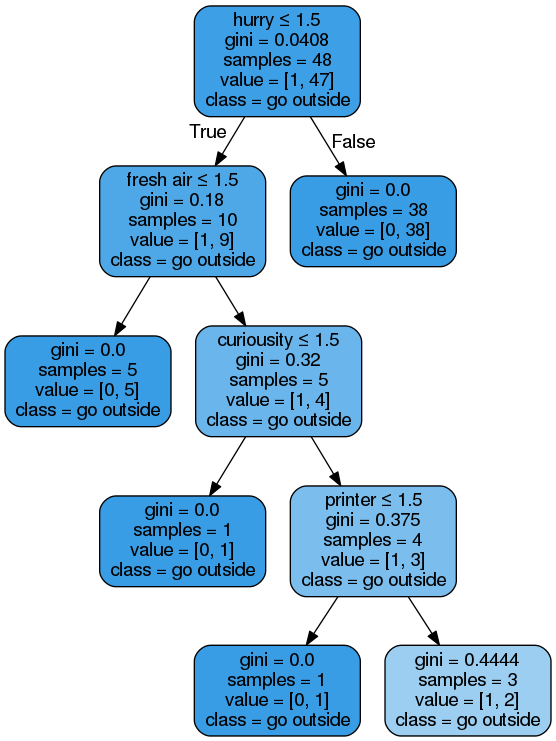
\includegraphics[width=0.7\columnwidth]{pics/decisionTree_8.png}
\caption{Decision tree for predicting if the route goes outside the building.}
\label{fig:dt8}
\end{figure*}

\begin{figure*}[!h]
\centering
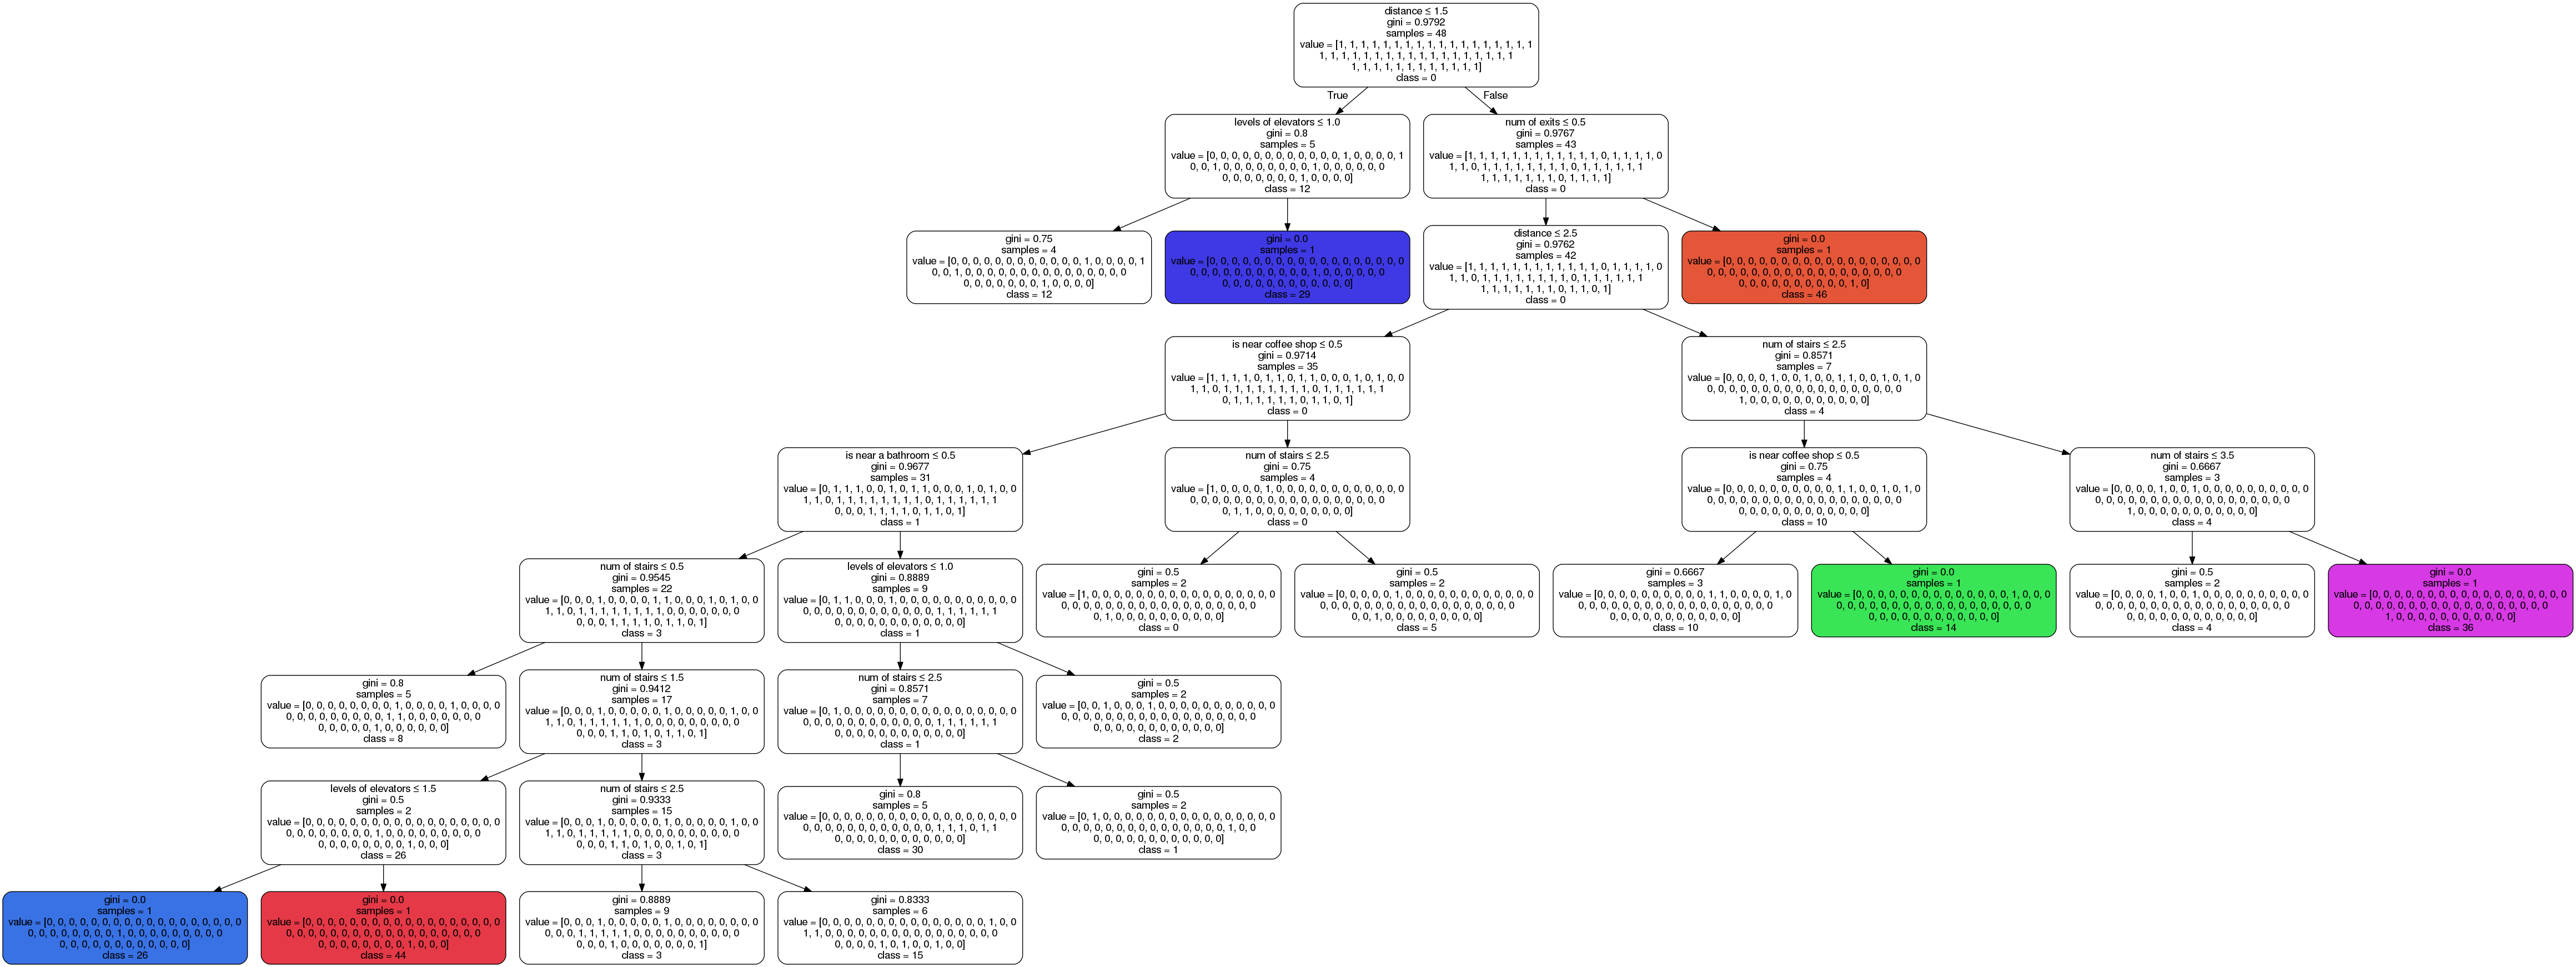
\includegraphics[width=1.0\columnwidth]{pics/routeDT.png}
\caption{Decision tree for predicting which route should be picked.}
\label{fig:dt9}
\end{figure*}


\section{DISCUSSION}
From the routeSuggestionDecisionTree, we can see that only a few of the routes are picked. These means that the number of potential routes is quite small since there are only limited possible routes. Besides, one route can fulfill many physical requirements. We think there are more physical properties which are useful. Also, it will be great if we can support more sources and destinations.


At the beginning, we asked the participants to draw the route before answering the survey questions. However, according to the participants, it will be more difficult for them to recall how they fill when they draw the route. Besides, they think taking the survey at first will be better. We adapt their suggestions and update our project to the current version.


Besides of the decision tree algorithm we used, the k-NN algorithm also seems to meet our requirements and is better when there are more features to be considered. It will be a good idea to implement a k-NN classifier for route suggesting problem. 

\section{CONCLUSION}
We design a new method to solve the in-building route suggesting problem. We take advantage of crowdsourcing to collect route data and corresponding user preferences. Based on the analysis, we derive 8 physical properties of the route which are critical to the choice of the route. With decision tree algorithm, we are able to classify the desired physical properties based on the user's preference and use the physical properties to predict which route is most suitable for a specific preference.

\section{FUTURE WORK}
Our current system only includes MC and DC on UW campus. In the future, we would like to extend our system to cover the entire UW campus. One of the important concepts of the system is crowdsourcing, thus via the extension of the entire campus, we will be able to collect many in-building routes. In the real scenario, not every student has the comprehensive building structure knowledge of the entire campus. For example, students in the Faculty of Mathematics are more familiar with MC, DC, M3, etc. while students in the Faculty of Engineering are more familiar with E2, E3, E5, etc. The reason is that students have frequent activities in those buildings, such as submitting assignments, attending professor’s office hours, etc. 


However, class locations issued by the Registrar are spread across the entire campus. People are willing to travel to their destinations through hallways or bridges connecting buildings especially in winter or when the weather condition is extremely harsh, such as heavy snow, rain, etc. 


Our system can really help to achieve people’s preference, which is traveling inside buildings through in-door connections to keep safe and warm. Since we have mentioned the fact that not every student has the comprehensive building structure knowledge of the entire campus, during the crowdsourcing stage, students record their in-building routes for the buildings they are mostly familiar with through our system, and provide personal preferences other than the outdoor conditions associating with the routes. Thus, the system will be able to gather enough in-building routes between building groups, covering the entire campus. What our system will do is that it combines several routes collected in the crowdsourcing stage to a single route from one location to another. Thus, the system can provide the user with one or more crowdsourced and processed in-building routes with personal preferences from the starting point to the destination. Here, personal preferences and starting/ending locations are inputted by the user.


\section{Acknowledgments}

We would like to thank Dr. Edith Law and everyone in CS889 class for their great help through this study.

\balance

\bibliographystyle{acm-sigchi}
\bibliography{report}
\end{document}
